\documentclass[
	% -- opções da classe memoir --
	12pt,				% tamanho da fonte
	openright,			% capítulos começam em pág ímpar (insere página vazia caso preciso)
	oneside,			% para impressão em verso e anverso. Oposto a oneside
	a4paper,			% tamanho do papel. 
	% -- opções da classe abntex2 --
	%chapter=TITLE,		% títulos de capítulos convertidos em letras maiúsculas
	%section=TITLE,		% títulos de seções convertidos em letras maiúsculas
	%subsection=TITLE,	% títulos de subseções convertidos em letras maiúsculas
	%subsubsection=TITLE,% títulos de subsubseções convertidos em letras maiúsculas
	% -- opções do pacote babel --
	english,			% idioma adicional para hifenização
	french,				% idioma adicional para hifenização
	spanish,			% idioma adicional para hifenização
	brazil				% o último idioma é o principal do documento
	]{abntex2}


% --- 
% CONFIGURAÇÕES DE PACOTES
% --- 
% ---
% Pacotes básicos 
% ---
\usepackage{lmodern}			% Usa a fonte Latin Modern			
\usepackage[T1]{fontenc}		% Selecao de codigos de fonte.
\usepackage[utf8]{inputenc}		% Codificacao do documento (conversão automática dos acentos)
\usepackage{lastpage}			% Usado pela Ficha catalográfica
\usepackage{indentfirst}		% Indenta o primeiro parágrafo de cada seção.
\usepackage{color}				% Controle das cores
\usepackage{graphicx}			% Inclusão de gráficos
\usepackage{microtype} 			% para melhorias de justificação
\usepackage{ufc-abntex2}
% ---
		
% ---
% Pacotes adicionais, usados apenas no âmbito do Modelo Canônico do abnteX2
% ---
\usepackage{lipsum}				% para geração de dummy text
% ---

% ---
% Pacotes de citações
% ---
\usepackage[brazilian,hyperpageref]{backref}	 % Paginas com as citações na bibl
\usepackage[alf]{abntex2cite}	% Citações padrão ABNT

% ---
% Configurações do pacote backref
% Usado sem a opção hyperpageref de backref
\renewcommand{\backrefpagesname}{Citado na(s) página(s):~}
% Texto padrão antes do número das páginas
\renewcommand{\backref}{}
% Define os textos da citação
\renewcommand*{\backrefalt}[4]{
	\ifcase #1 %
		Nenhuma citação no texto.%
	\or
		Citado na página #2.%
	\else
		Citado #1 vezes nas páginas #2.%
	\fi}%
% ---

% ---
% Configurações de aparência do PDF final

% alterando o aspecto da cor azul
\definecolor{blue}{RGB}{41,5,195}

% informações do PDF
\makeatletter
\hypersetup{
     	%pagebackref=true,
		pdftitle={\@title}, 
		pdfauthor={\@author},
    	pdfsubject={\imprimirpreambulo},
	    pdfcreator={LaTeX with abnTeX2},
		pdfkeywords={abnt}{latex}{abntex}{abntex2}{trabalho acadêmico}, 
		colorlinks=true,       		% false: boxed links; true: colored links
    	linkcolor=blue,          	% color of internal links
    	citecolor=blue,        		% color of links to bibliography
    	filecolor=magenta,      		% color of file links
		urlcolor=blue,
		bookmarksdepth=4
}
\makeatother
% --- 

% --- 
% Espaçamentos entre linhas e parágrafos 
% --- 

% O tamanho do parágrafo é dado por:
\setlength{\parindent}{1.3cm}

% Controle do espaçamento entre um parágrafo e outro:
\setlength{\parskip}{0.2cm}  % tente também \onelineskip

% ---
% compila o indice
% ---
\makeindex
% ---


% Preambulo (Editar para mudar as variaveis do documento)
%
% Documento: Preâmbulo
%

\instituicao{Universidade Estadual do Sudoeste da Bahia}
\sigla{UESB}
\campus{Campus de Vitória da Conquista}
\local{Vitória da Conquista, Bahia}
\curso{Curso de Ciência da Computação}
\autor{Matheus Coqueiro Andrade}
\titulo{Estudo de caso sobre a utilização da Tecnologia da Informação Verde na Universidade Estadual do Sudoeste da Bahia}
%\subtitulo{Um estudo e aplicação}
\data{2018}
%\grau{Bacharel}
\dataapresentacao{29/06/2018}

%Dados Orientador
\orientador{Gidevaldo Novais Dos Santos}
\instOrientador{Universidade Estadual do Sudoeste da Bahia}
\departamentoorientador{Campus Vitória da Conquista}
\titulacaoorientador{Prof. Me.}

%Dados Coorientador
%\coorientador{Debra Morgan}
%\instCoorientador{Universidade Federal de Alagoas}
%\departamentocoorientador{Campus Arapiraca}
%\titulacaocoorientador{Prof. Me.}

%Dados Examinador 1
\nomeexamum{Helio Lopes Dos Santos}
\instexamum{Universidade Estadual do Sudoeste da Bahia}
\departamentoexamum{Campus Vitória da Conquista}
\titulacaoexamum{Prof. Dr.}

%Dados Examinador 2
\nomeexamdois{Roque Mendes Prado Trindade}
\instexamdois{Universidade Estadual do Sudoeste da Bahia}
\departamentoexamdois{Campus Vitória da Conquista}
\titulacaoexamdois{Prof. Dr.}

\tipotrabalho{Trabalho de Conclusão de Curso (Monografia)}
\preambulo{Trabalho de Conclusão de Curso apresentado como  requisito  parcial  para  obtenção  do grau de Bacharel em Ciência da Computação da  \imprimirinstituicao - \imprimirsigla, \imprimircampus.}


\begin{document}
\frenchspacing 

% ----------------------------------------------------------
% ELEMENTOS PRÉ-TEXTUAIS
% ----------------------------------------------------------
% \pretextual
% Capa
\imprimircapa
% Folha de rosto (* indica que haverá a ficha bibliográfica)
\imprimirfolhaderosto*

% Ficha Bibliográfica
% ---
% Inserir a ficha bibliografica
% ---

% Isto é um exemplo de Ficha Catalográfica, ou ``Dados internacionais de
% catalogação-na-publicação''. Você pode utilizar este modelo como referência. 
% Porém, provavelmente a biblioteca da sua universidade lhe fornecerá um PDF
% com a ficha catalográfica definitiva após a defesa do trabalho. Quando estiver
% com o documento, salve-o como PDF no diretório do seu projeto e substitua todo
% o conteúdo de implementação deste arquivo pelo comando abaixo:
%
% \begin{fichacatalografica}
%     \includepdf{fig_ficha_catalografica.pdf}
% \end{fichacatalografica}
\begin{fichacatalografica}
	\vspace*{\fill}					% Posição vertical
	\hrule							% Linha horizontal
	\begin{center}					% Minipage Centralizado
	\begin{minipage}[c]{12.5cm}		% Largura
	
	\imprimirautor
	
	\hspace{0.5cm} \imprimirtitulo  / \imprimirautor. --
	\imprimirlocal, \imprimirdata.
	
	\hspace{0.5cm} \pageref{LastPage} p. : il. (algumas color.) ; 30 cm.\\
	
	\hspace{0.5cm} \imprimirorientadorRotulo~\imprimirorientador\\
	
	\hspace{0.5cm}
	\parbox[t]{\textwidth}{\imprimirtipotrabalho~--~\imprimirinstituicao
	\par
	\imprimircampus
	\par
	Curso de \imprimircurso,
	\imprimirdata.}\\
	
	\hspace{0.5cm}
		1. TI Verde.
		2. Sustentabilidade.
		I. \imprimirorientador.
		II. \imprimirinstituicao.
		III. \imprimircurso.
		IV. \imprimirtitulo\\ 			
	
	\hspace{8.75cm} CDU 02:141:005.7\\
	
	\end{minipage}
	\end{center}
	\hrule
\end{fichacatalografica}
% ---

% Errata
%\include{editaveis/errata}

% Folha de Aprovação
% ---
% Inserir folha de aprovação
% ---

% Isto é um exemplo de Folha de aprovação, elemento obrigatório da NBR
% 14724/2011 (seção 4.2.1.3). Você pode utilizar este modelo até a aprovação
% do trabalho. Após isso, substitua todo o conteúdo deste arquivo por uma
% imagem da página assinada pela banca com o comando abaixo:
%
% \includepdf{folhadeaprovacao_final.pdf}
%
\begin{folhadeaprovacao}

  \begin{center}
    {\bfseries\Large\imprimirautor}
    \vspace{1cm}

    \begin{center}
      \bfseries\Large\imprimirtitulo
    \end{center}

    \vspace{2cm}
    \begin{minipage}{\textwidth}
        \imprimirpreambulo
        \\ \\ \\
        Aprovada em: \imprimirdataapresentacao
    \end{minipage}%
     
    \vspace{2cm}
	\textbf{BANCA EXAMINADORA}
	
	\vspace*{1.2 cm}%Espaçamento entre linhas
    \rule{9 cm}{.1 mm}\\
    {\imprimirtitulacaoorientador}{ }{\imprimirorientador}\\
    {\imprimirinstOrientador}\\
    {\imprimirdepartamentoorientador}\\
    Orientador\\

    \vspace*{1.1 cm}%Espaçamento entre linhas
    \rule{9 cm}{.1 mm}\\
    \imprimirtitulacaoexamum{ }\imprimirnomeexamum\\
    \imprimirinstexamum\\
    \imprimirdepartamentoexamum\\
    Examinador\\

    \vspace*{1.1 cm}%Espaçamento entre linhas
    \rule{9 cm}{.1 mm}\\				
    				
    \imprimirtitulacaoexamdois{ }\imprimirnomeexamdois\\
    \imprimirinstexamdois\\
    \imprimirdepartamentoexamdois\\
    Examinador
    \vspace*{1.3 cm}%Espaçamento entre linhas
   \end{center}
  
\end{folhadeaprovacao}
% ---

%\imprimirfolhadeaprovacao

% Dedicatória
% ---
% Dedicatória
% ---

\begin{dedicatoria}
   \vspace*{\fill}
   	\begin{flushright}
   \noindent
   Este trabalho é dedicado aos meus pais, que foram o meu porto seguro e me deram todo o suporte possível para que eu chegasse até o final.
   	\end{flushright}
\end{dedicatoria}
% ---

% Agradecimentos
% ---
% Agradecimentos
% ---
\begin{agradecimentos}
  %
  %   Editar ainda!!!
  %

  Aos meus pais. 

  Agradeço à minha namorada Rafaela Oliveira.

  Amigos Especiais (Maioli, Yuri e Wanderson).

  Colegas de turma, curso em especial ao Lindalva.

  Aos professores, em especial ao professor roque, marco antônio e alzira.

  À celina.

  Aos meus amigos que ficaram pelo meio do caminho, Iury Simmont, Jade Dias, Laherce, Matheus Couto, Pedro Barros e Raveni, vocês foram mais que meus amigos, foram a minha família. 
\end{agradecimentos}
% ---

% Epígrafe
% ---
% Epígrafe
% ---
\begin{epigrafe}
    \vspace*{\fill}
	\begin{flushright}
		\textit{``Para ter sucesso neste mundo não basta ser \\
		estúpido, é preciso também ter boas maneiras\\
		(Voltaire)}
	\end{flushright}
\end{epigrafe}
% ---

% Resumo
% resumo em português
\setlength{\absparsep}{18pt} % ajusta o espaçamento dos parágrafos do resumo
\begin{resumo}
 Segundo a NBR6028:2003, o resumo deve ressaltar o
 objetivo, o método, os resultados e as conclusões do documento. A ordem e a extensão
 destes itens dependem do tipo de resumo (informativo ou indicativo) e do
 tratamento que cada item recebe no documento original. O resumo deve ser
 precedido da referência do documento, com exceção do resumo inserido no
 próprio documento. (\ldots) As palavras-chave devem figurar logo abaixo do
 resumo, antecedidas da expressão Palavras-chave:, separadas entre si por
 ponto e finalizadas também por ponto.

 \textbf{Palavras-chaves}: latex. abntex. editoração de texto.
\end{resumo}

% Abstract
% resumo em inglês
\begin{resumo}[Abstract]
 \begin{otherlanguage*}{english}
 

   \vspace{\onelineskip}
 
   \noindent 
   \textbf{Key-words}: latex. abntex. text editoration.
 \end{otherlanguage*}
\end{resumo}

% Lista de ilustrações
\pdfbookmark[0]{\listfigurename}{lof}
\listoffigures*
\cleardoublepage

% Lista de tabelas
\pdfbookmark[0]{\listtablename}{lot}
\listoftables*
\cleardoublepage

% Abreviaturas e Siglas
% Lista de abreviaturas e siglas
% ---
\begin{siglas}
    \item[AGESPI]   Assessoria na Gestão de Projetos e Convênios Institucionais
    \item[AIIM]	    \textit{Association for Information and Image Management}
    \item[APG]	    Assessoria de Gestão de Pessoas
    \item[CEUAS]	Centro Universitário de Atenção à Saúde
    \item[CRM]	    \textit{Costumer Relationship Management}
    \item[DLL]	    \textit{Dynamic Link Library}
    \item[EAI]	    \textit{Enterprise Apliccation Integration}
    \item[EPA]	    \textit{Environmental Protection Agency}
    \item[ERM]  	\textit{Enterprise Report Management}
    \item[FAINOR]	Faculdade Independente do Nordeste
    \item[FTC]  	Faculdade de Tecnologia e Ciências
    \item[ERP]	    \textit{Enterprise Resource Planning}
    \item[GED]	    Gestão Eletrônica de Documentos
    \item[IFBA]	    Instituto Federal da Bahia
    \item[PCF]	    Posto de Cadastro de Fornecedores
    \item[PDM]	    \textit{Product Data Management}
    \item[PEN]	    Processo Eletrônico Nacional
    \item[PID]  	Plano de Desenvolvimento Institucional
    \item[Procel]	Programa Nacional de Conservação de Energia Elétrica
    \item[REEE]	    Resíduos de Equipamentos Eletroeletrônicos
    \item[RH]   	Recursos Humanos
    \item[RoHS]	    \textit{Restriction of Certain Hazardous Substances}
    \item[RSE]  	Responsabilidade Social Empresarial
    \item[SEI]  	Sistema Eletrônico de Informação
    \item[SGA]  	Sistema de Gestão Ambiental
    \item[SIF]  	Setor de Informações Funcionais
    \item[TI]   	Tecnologia da Informação
    \item[TI Verde]	Tecnologia da Informação Verde
    \item[TIC]  	Tecnologia da Informação e Comunicação
    \item[TRF4]	    Tribunal Regional Federal da 4a Região
    \item[UESB]	    Universidade Estadual do Sudoeste da Bahia
    \item[UFBA]	    Universidade Federal da Bahia
    \item[UINFOR]	Unidade Organizacional de Informática
    \item[VDI]	    \textit{Virtual Desktop Infrastructure}
    \item[WEEE]	    \textit{Waste Electrical and Electronic Equipment Directive}
    
    

\end{siglas}
% ---

% Símbolos
%%Lista de símbolos
% ---
\begin{simbolos}
  \item[$ \Gamma $] Letra grega Gama
  \item[$ \Lambda $] Lambda
  \item[$ \zeta $] Letra grega minúscula zeta
  \item[$ \in $] Pertence
\end{simbolos}
% ---

% Sumário
\pdfbookmark[0]{\contentsname}{toc}
\tableofcontents*
\cleardoublepage

% ----------------------------------------------------------
% ELEMENTOS TEXTUAIS
% ----------------------------------------------------------
\textual

% ----------------------------------------------------------
% PARTE I
% ----------------------------------------------------------
\part{Preparação da pesquisa}

%
% Documento: Introdução
%

\chapter{Introdução}\label{chap:introducao}

Em tempos de globalização econômica e de comunicação, é de suma importância pensar nas gerações futuras. Segundo o relatório de \citeonline{brundtland1987report}, o ``desenvolvimento sustentável é o desenvolvimento que satisfaz as necessidades do presente sem comprometer a capacidade das futuras gerações satisfazerem suas próprias necessidade''. 

Para \citeonline{hart1995natural}, o desenvolvimento sustentável está relacionado com o crescimento sem prejuízos aos recursos naturais utilizados, onde a preocupação com os fatores ambientais são prioridade. 

Para as empresas e instituições, fica clara a necessidade de se adotar estratégias e modelos para se adequar ao desenvolvimento sustentável, a Tecnologia da Informação Verde (TI Verde).


%essa frase ficou longa pra caralho eu achei. Eu quebraria depois do "TI verde" e colocaria nessa pegada:
%(...) sobre a importância de se implementar modelos de Tecnologia da Informação Verde. Outra justificativa é o alto consumo de energia nesse tipo de instituição, que pode ser atacado por meio de uma série de vantagens da TI Verde, pois já existem dispositivos (...)
\section{Justificativa}

Hoje a Universidade Estadual do Sudoeste da Bahia (UESB) é a maior instituição de ensino da Mesorregião do Centro-Sul Baiano. Ela possui grande influência na comunidade local, tendo a responsabilidade social de implementar práticas sustentáveis e possuir um Sistema de Gestão Ambiental, tornando-se referência de sustentabilidade no âmbito tecnológico, criando uma iniciativa nesta área que atualmente é pouca explorada. Com isso, existe a chance de se conscientizar os gestores das demais instituições de ensino e empresas, sobre a importância, vantagens e ganhos, de se aplicar práticas verdes. 

\section{Questão da pesquisa}
Nos dias atuais, existe uma necessidade das organizações pensarem em maneiras de otimizar o uso das tecnologias, de modo que contribuam com a sustentabilidade e o desenvolvimento sustentável, minimizando os riscos e impactos ambientais e atendendo às dimensões da sustentabilidade (ambiental, social e econômica). Neste contexto, existem as seguintes questões que esta pesquisa tentará resolver:
\begin{itemize}
    \item Como a Tecnologia da Informação Verde é utilizada na Universidade Estadual do Sudoeste da Bahia, campus de Vitória da Conquista?
    \item A Universidade Estadual do Sudoeste da Bahia utiliza a Tecnologia da Informação Verde de maneira correta?
    \item Como a Tecnologia da Informação Verde pode ser aplicada na Universidade Estadual do Sudoeste da Bahia, visando ter uma redução no consumo de energia, geração de Resíduos de Equipamentos Eletroeletrônicos e gasto com a manutenção?
\end{itemize}

\section{Objetivo geral}
Apresentar os benefícios de utilizar práticas da Tecnologia da Informação Verde, contribuindo para a diminuição dos riscos ou dos impactos ambientais causados pela má utilização da tecnologia, além da redução dos gastos. 

\section{Objetivos específicos}
Realizar um estudo sobre a TI Verde, verificando as soluções que visam o melhor uso da tecnologia da informação, garantindo à redução dos impactos ambientais.
 
Analisar a utilização da TI Verde na Unidade Organizacional de Informática da UESB, campus de Vitória da Conquista.  

Propor novas soluções baseadas nas práticas da TI Verde, apresentando os ganhos que a instituição terá por implementar essas soluções.


\section{Metodologia}

\subsection{Tipo de pesquisa}
A modalidade desta pesquisa é de campo e bibliográfica. Quanto aos objetivos é do tipo exploratória e descritiva, e quanto à forma de abordagem é qualitativa, com aplicação de entrevista estruturada, entrevista semiestruturada e de um questionário.

\subsection{Campo de pesquisa}

A entrevista semiestruturada e o questionário foram aplicadas com o diretor da Unidade Organizacional de Informática da UESB (UINFOR). A entrevista foi realizada no dia 15 de Junho de 2018, utilizando o aplicativo de mensagens instantâneas \textit{WhatsApp Messenger}, já o questionário foi aplicado no dia 17 de Abril de 2018, utilizando o editor de texto online Google Documentos. Também foi realizado a leitura do Roteiro de Diagnóstico Setorial, disponibilizado pelo entrevistado, que descreve todas as funções, atribuições, atividades, estruturas e processos da UINFOR, além do Plano de Desenvolvimento Institucional (PID) 2013-2017$^{[}$\footnote{PID 2013-2017, Disponível em: \url{http://www.uesb.br/pdi/arquivos/PDI_Final.pdf}.  Acessado em 16 de junho de 2018}$^{]}$ que contém diversas informações sobre a UESB.

A entrevista estruturada foi aplicada com o analista e desenvolvedor do projeto de Gestão Eletrônica de Documentos (GED), do Setor de Informações Funcionais (SIF). A entrevista foi realizada no dia 14 de Junho de 2018, utilizando o editor de texto online Google Documentos e o aplicativo de mensagens instantâneas \textit{WhatsApp Messenger}.

\subsection{Coleta de dados}
A obtenção de dados relacionados ao estudo de caso foi realizada mediante aplicação de um questionário (Apêndice A), uma entrevista semiestruturada (Apêndice B) e uma entrevista estruturada (Apêndice C). As perguntas das entrevistas foram elaboradas pelo pesquisador a partir do conhecimento obtido pelo referencial teórico, se baseando em alguns trabalhos estudados. Foram contemplados tópicos considerados de relevância para o tema pelo pesquisador, a fim de coletar dados no que se refere à utilização da TI verde pela instituição, de modo que se possa medir o grau de adequação com base nas respostas encontradas.

O questionário aplicado foi extraído de \citeonline{lunardi2014desenvolvimento}, e serve para avaliar o grau de utilização da TI Verde pelas organizações. Ele é dividido em 5 fatores, apresentados a seguir: 
\begin{itemize}
    \item  \textbf{Consciência socioambiental:} Avalia se a organização está consciente da necessidade de abordar as questões ambientas de forma mais proativa;
    \item \textbf{Ações sustentáveis:} Avalia se a organização implementa iniciativas para tornar os processos o mais sustentável possível;
    \item \textbf{\textit{Expertise} ambiental:} Avalia se a organização se submete a experimentar, atualizar e buscar novas abordagens, informações e conhecimentos a fim de aplicar estratégias sustentáveis na área de Tecnologia da Informação;
    \item \textbf{Monitoramento:} Avalia se a organização gerencia as atividades e medidas de Tecnologia da Informação voltadas à redução do consumo de recursos e dos danos ao meio ambiente;
    \item \textbf{Orientação ambiental:} Avalia se a organização está comprometida com a sustentabilidade e com o suporte às inovações ambientais.
\end{itemize}

As informações para o embasamento teórico foram coletadas através de fontes primárias como livros, artigos, monografias e leis sobre o referido tema, e fontes complementares, como sites da internet. 

Após a coleta de dados, foi identificada e medida à utilização da TI Verde, e propostas novas soluções para serem utilizadas pela instituição.

\subsection{Estrutura de desenvolvimento}
A estrutura de desenvolvimento do projeto de pesquisa foi dividido nas seguintes etapas:

\begin{itemize}
  \item Realizar um estudo sobre a TI Verde;
  \item Pesquisar e conhecer como a TI Verde é utilizada atualmente na UESB, em Vitória da Conquista;
  \item Identificar as maiores necessidades e problemas relacionados à Tecnologia da Informação que a UESB enfrenta;
  \item Propor soluções baseadas nas práticas de TI Verde;
  \item Apresentar uma conclusão sobre a utilização de TI Verde na UESB.
\end{itemize}


\section{Estrutura do trabalho}

% ----------------------------------------------------------
% PARTE II
% ----------------------------------------------------------
\part{Referencial teórico}

%
% Documento: Tecnologia de Informação Verde
%

\chapter{Tecnologia da Informação Verde}

\section{Informação}

De acordo com \citeonline{pinheiro2004informaccao}, a informação é dependente de um contexto (científico, tecnológico, industrial, artístico, cultural, entre outros). Segundo \citeonline[p. 17]{aguilar2009tecnologia}, a informação corresponde a grupos de dados classificados e organizados, que tenham valor para que uma pessoa ou empresa consiga utilizar para seu benefício. Na vida real ou empresarial, dispor de informação é um fator determinante para o sucesso e seu mal-uso pode trazer prejuízos astronômicos. Para ajudar a resolver esses problemas existe o que chamam de Tecnologia da Informação (TI).

\section{Tecnologia da Informação}

A evolução humana tem ligação direta com o avanço da tecnologia, bem como o contrário. Um é inerente ao outro e isso é indiscutível quando observamos as várias mudanças nos instrumentos, que se tornaram mais funcionais, acompanhando a evolução do homem, tanto na anatomia de seu corpo, principalmente de sua mão, quanto em seu cérebro. \cite[p. 107-111]{acevedo1998ciencia}. Ela foi desenvolvida para satisfazer as necessidades humanas e já existia antes dos homens e dos conhecimentos científicos e mesmo assim foi capaz de criar estruturas e instrumentos complexos. \cite{acevedo1998ciencia, veraszto2004projeto}. 

Para \citeonline[p. 2]{de1996tecnologia}, a tecnologia pode ser definida como conjunto de conhecimentos, de sua maioria científicos, que são aplicados em determinados ramos de atividades. Podendo ser considerada uma ciência que trata da técnica.

A TI é um dos campos da tecnologia que tomou força no século XX. Surgiu como um meio para melhorar os processos de criação e desenvolvimento \cite[p. 2]{de1996tecnologia}, e atualmente é um forte indicador de melhoria na performance e produtividade \cite[p. 2]{lunardi2001efeitos}, além de ter grande relevância na continuação de esforços das empresas para tornarem os seus processos mais ágeis e produtivos \cite{shaw1997information}. Seu grande papel é o gerenciamento de informações, mas nem sempre esse gerenciamento se dá de forma agradável para o meio ambiente \cite[p. 6-7]{silva2011}. Para solucionar os problemas e amenizar os impactos decorrentes da tecnologia de informação pesquisadores desenvolveram as práticas da Tecnologia da Informação Verde.

\section{Tecnologia da Informação Verde}

O grande avanço tecnológico dos últimos anos, acompanhado da obsolescência programada dos produtos e do consumo desenfreado com consequente produção em grande escala resultam em grandes riscos para o meio ambiente. O descarte inadequado do lixo eletroeletrônico tem grande impacto ambiental e traz sérios riscos à saúde humana, uma das causas é a contaminação de solos e águas com minérios pesados. Há também o grande gasto de energia, uma vez que o número de aparelhos eletrônicos vem crescendo em empresas e indústrias além de vários serviços que são utilizados 24h horas por dia ou são atualizados sempre, impedindo seu desligamento durante a noite ou fins de semana.

Segundo \citeonline[p. 2]{laurindo2000estudo}, a tecnologia “não só sustenta as estratégias de negócio existentes, mas também permite que se viabilizem novas estratégias empresariais”. Uma dessas novas estratégias surgiu com a busca pela redução dos impactos ambientais e a possível reversão de danos causados, o que resultou no estabelecimento de práticas sustentáveis na área de TI, que juntas são conhecidas como TI Verde. \cite{aguilar2009tecnologia}.

A TI Verde vem do conceito de ecoeficiência, e teve origem na década de 80, e se consiste do uso eficiente dos recursos naturais, e na última década vem sendo utilizado com frequência nos setores de TI. \cite{ferreira2009tiverde}. Atualmente, a TI Verde pode ser definida como um conceito que as empresas de tecnologia criaram para agregar o uso de recursos tecnológicos e políticas que minimizem cada vez mais as agressões ao meio ambiente. \cite{briefing2008preciso}.

\begin{citacao}
A TI Verde é o estudo e a prática de projetar, fabricar,
usar e descartar computadores, servidores e subsistemas associados (monitores, impressoras, dispositivos de armazenamento e de rede e sistemas de comunicação), de forma eficiente e eficaz, com o mínimo de impacto para o meio ambiente, lutando para atingir a viabilidade econômica e melhorar o uso e o desempenho dos sistemas e respeitando as responsabilidades sociais e éticas. \cite{lunardi2014desenvolvimento}.
\end{citacao} 

Para \citeonline[p. 36]{aguilar2009tecnologia}, a economia de energia e corte de gastos sempre foram as grandes preocupações das empresas. Essa preocupação se torna ainda maior na área de TI, pois os \textit{datacenters} geralmente costumam figurar como a maior porcentagem dos gastos de energia elétrica de uma companhia, já que em um banco, por exemplo, a energia que a TI utiliza pode superar a metade de todo consumo.  

Além da preocupação com o meio ambiente, várias dessas práticas têm um impacto econômico positivo, o que contribui para sua ampla adoção, já que a busca pelo aumento da produtividade passa pela redução de gastos e tem influência direta da utilização de recursos básicos, como água, energia e matérias primas.

\section{Tecnologia da Informação Verde nas organizações}

Para \citeonline{kraemer2005responsabilidade} o fator ambiental vem mostrando a necessidade de adaptação das organizações e consequentemente direcionando novos caminhos na sua expansão. As organizações precisam alterar seus paradigmas, mudando sua visão empresarial, objetivos, estratégias de investimentos e de marketing, se adaptando à nova realidade do mercado global e ecologicamente correto.

\begin{citacao}
As empresas têm um papel extremamente relevante. Através de uma prática empresarial sustentável, provocando mudança de valores e de orientação em seus sistemas operacionais, estarão engajadas à ideia de desenvolvimento sustentável e preservação do meio ambiente \cite[p. 3]{kraemer2005responsabilidade}. 
\end{citacao}

Os desequilíbrios sócio-ambientais são o resultado do velho paradigma cartesiano e mecanicista, com sua visão fragmentada do mundo \cite[p. 28]{almeida2002bom}. Este paradigma é meramente capitalista e visa o lucro máximo, fazendo com que o meio ambiente seja apenas um bem privado, no que se refere à produção e descarte dos seus resíduos. Este modelo não é sustentável ao longo do tempo, pois ficou claro que os recursos naturais são esgotáveis e, portanto, finitos, se mal utilizados \cite{kraemer2005responsabilidade}.

A \autoref{tab:cartesiano-sustentabilidade} apresenta uma comparação do paradigma atual com o paradigma sustentável.

\begin{table}[htb]	
    \ABNTEXfontereduzida
	\Caption{\label{tab:cartesiano-sustentabilidade} Paradigma cartesiano \textit{versus} paradigma da sustentabilidade.}
	\UECEtab{}{
		\begin{tabular}{p{7cm}p{8cm}}
			\toprule
    		\textbf{Cartesiano} & \textbf{Sustentável} \\
			\midrule \midrule
				Reducionista, mecanicista, tecnocêntrico  & Orgânico, holístico, participativo \\
				Fatos e valores não relacionados & Fatos e valores fortemente relacionados \\
				Preceitos éticos desconectados das práticas cotidianas & Ética integrada ao cotidiano \\
				Separação entre o objetivo e o subjetivo & Interação entre o objetivo e o subjetivo \\
				Seres humanos e ecossistemas separados, em uma relação de dominação & Seres humanos inseparáveis dos ecossistemas, em uma relação de sinergia \\
				Conhecimento compartimentado e empírico  & Conhecimento indivisível, empírico e intuitivo \\
				Relação linear de causa e efeito & Relação não-linear de causa e efeito \\
				Natureza entendida como descontínua, o todo formado pela soma das partes  & Natureza entendida como um conjunto de sistemas inter-relacionados, o todo maior que a soma das partes \\
				Bem-estar avaliado por relação de poder (dinheiro, influência, recursos)  & Bem-estar avaliado pela qualidade das inter-relações entre os sistemas ambientais e sociais \\
				Ênfase na quantidade (renda per capita) & Ênfase na qualidade (qualidade de vida) \\
				Análise & Síntese \\
				Centralização de poder & Descentralização de poder \\
				Especialização & Transdisciplinaridade \\
				Ênfase na competição & Ênfase na cooperação \\
				Pouco ou nenhum limite tecnológico  & Limite tecnológico definido pela sustentabilidade \\
			\bottomrule
		\end{tabular}
	}{
		\Fonte{\citeonline{almeida2002bom}}
    }
\end{table}

\subsection{Responsabilidade Social}

O Governo vem pressionando cada vez mais as organizações para que desenvolvam práticas para reduzir seus impactos ambientais e sociais. Recentemente, houveram grandes progressos quanto à conscientização sobre a responsabilidade social e maior compreensão dos desafios da sustentabilidade \cite{kraemer2005responsabilidade}.

A Responsabilidade Social Empresarial (RSE) pode ser conceituada através da integração das preocupações sociais e ambientais em suas operações e interação com todas as partes interessadas. É caraterizada pela sua adoção voluntária, para além das prescrições legais. Este conceito é associado com o de desenvolvimento sustentável, onde as organizações integram em suas operações o impacto econômico, social e ambiental \cite{biorumo}.  

A RSE conta com três fatores fundamentais: o planeta (preocupações ambientais), as pessoas (preocupações sociais) e a rentabilidade (preocupações econômicas), esta tridimensionalidade é definida pela expressão \textit{Triple Bottom Line}, apresentada na figura \autoref{fig_triple_bottom_line} \cite{biorumo}.


\begin{figure}[htb]
    \caption{\label{fig_triple_bottom_line}\textit{Triple Bottom Line}.}
    \begin{center}
        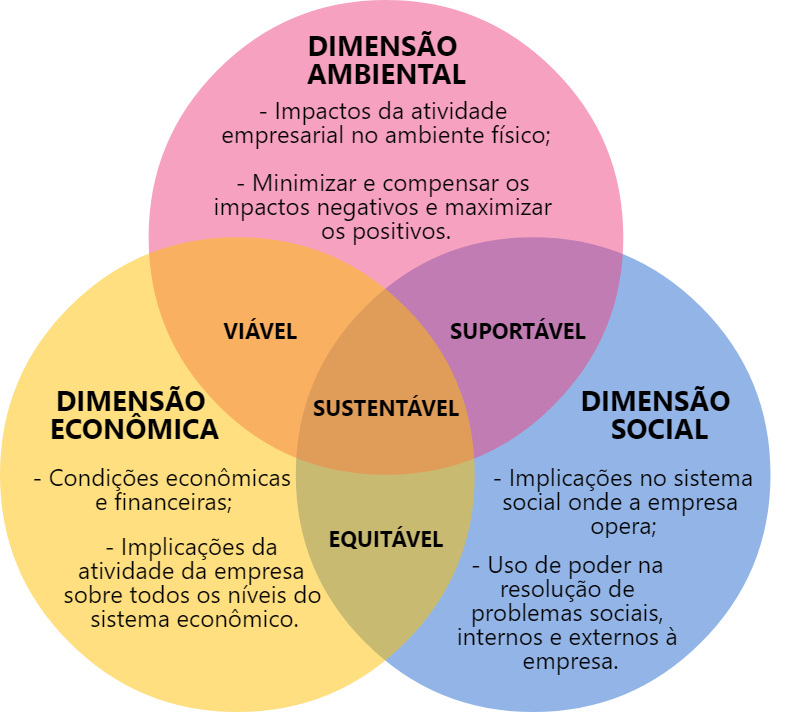
\includegraphics[scale=0.45]{imagens/triple-bottom-line.png}
    \end{center}
    \FonteFigura{Adaptado de \citeonline[p. 24]{biorumo}.}
\end{figure}

\subsection{Gestão Ambiental}

Alguma coisa...

\section{As práticas de TI Verde}

%As práticas de TI Verde, nos dias atuais, são utilizadas como estratégias de negócio na maior parte das grandes das empresas. Elas garantem lucros, bem-estar e reconhecimento da empresa, além de ajudar na proteção do meio ambiente, melhorando o futuro das próximas gerações, tornando-se imprescindível no dia a dia de qualquer empresa.%

A adoção de práticas sustentáveis é bem vista e traz maior reconhecimento para as organizações que as utilizam, pois, a sociedade atual se preocupa com a preservação do meio ambiente. \cite{abreu2012ti}. Essas práticas são aplicadas de acordo com cada perfil de organização. Nos dias atuais, é indispensável uma análise estrutural da empresa para identificar qual prática mais se adéqua a sua realidade. A implementação dessas práticas trará benefícios tanto para o meio ambiente, como também para a empresa. \cite{pinto2011estudo}.

Estas práticas envolvem ações diversas com o objetivo de economizar recursos e aumentar a durabilidade dos equipamentos usados.  São elas economia de energia, virtualização de servidores e \textit{desktop}, videoconferência, economia de papel e descarte, e reciclagem de REEE. Com o avanço tecnológico surgirão novas práticas de TI Verde para que o uso da TI se torne sustentável \cite[p. 8]{pinto2011estudo}.

\subsection{Os três níveis}

\citeonline{takahashi2009ti} e \citeonline[p. 7]{pinto2011estudo} classificam as práticas de TI Verde em três níveis:

\subsubsection{TI Verde Tático}

Nesse nível as práticas implementadas não modificam a infraestrutura nem interferem nas políticas internas do local, além de não gerarem custos adicionais. Abrangem mudanças ligadas à economia de recursos e tem como medidas o controle do uso excessivo de energia elétrica de uma organização. Alguns exemplos são o monitoramento automático do gasto de energia dos equipamentos, desligando-os quando estão em desuso, o uso de lâmpadas mais eficientes e a mudança na organização e disposição dos equipamentos para melhor circulação e consequente dissipação do calor, otimizando assim a temperatura das salas.

\subsubsection{TI Verde Estratégico}

Nesse nível as mudanças realizadas envolvem a convocação de uma auditoria da infraestrutura de TI e do seu uso relacionado ao meio ambiente e novos meios de produção de bens ou serviços são desenvolvidos e implementados de maneira ecológica. São criadas novas políticas internas e medidas de controle e descarte dos REEE. A adoção destas medidas geram um \textit{marketing} positivo, melhorando assim a imagem dessa organização diante da sociedade. Algumas práticas realizadas neste nível, diferentemente do anterior, geram um custo adicional devido a criação de uma nova rede elétrica visando uma maior eficiência energética e de sistemas computacionais que tenham um menor consumo elétrico, por meio da substituição dos equipamentos por outros mais econômicos e possíveis reformas estruturais.

\subsubsection{TI Verde a Fundo}

Esse nível é a integração dos níveis anteriores. É necessário a criação de um projeto de total modificação estrutural para maximizar a economia de energia e a sustentabilidade da organização. São realizadas grandes mudanças na infraestrutura que visam o otimizar o desempenho dos equipamentos e a padronização dos processos, como projetos de sistemas de refrigeração, iluminação e disposição de equipamentos, gerando um alto custo para a sua implementação.

\subsection{Virtualização}

A virtualização é uma técnica utilizada para emular um ambiente computacional sobre outro, ela é bastante popular na maioria das organizações, pois ela reduz aumento do número de maquinas físicas quando se tem uma diversidade de sistemas operacionais. As máquinas virtuais\footnote{Nome dado para ambientes computacionais simulados} podem ter múltiplas instâncias em um mesmo \textit{hardware} e incluem as bibliotecas do sistema operacional desejado, proporcionando um uso eficiente do seu poder de processamento e um alto grau de portabilidade. A redução de maquinas físicas implica na queda dos gastos da infraestrutura, como espaço, energia elétrica, cabeamento, refrigeração, suporte e manutenção de vários sistemas \cite[p. 174-175]{carissimi2008virtualizaccao}.

\citeonline[p. 193]{carissimi2008virtualizaccao} e \citeonline[p. 163-165]{neto2015ti} apresentam os seguintes métodos de virtualização oferecidos pela \textit{Microsoft}:
\begin{itemize}
    \item Virtualização de Servidor: as máquinas virtuais são criadas através de um software onde as mesmas emulam servidores, permitindo a execução dos seus sistemas operacionais de maneira simultânea. Dois ou mais servidores virtuais são emulados em um único servidor físico, otimizando o uso da memória, processamento e armazenamento (\autoref{fig_virt_serv});
    
    \begin{figure}[htb]
    	\caption{\label{fig_virt_serv}Virtualização de Servidores.}
    	\begin{center}
    	    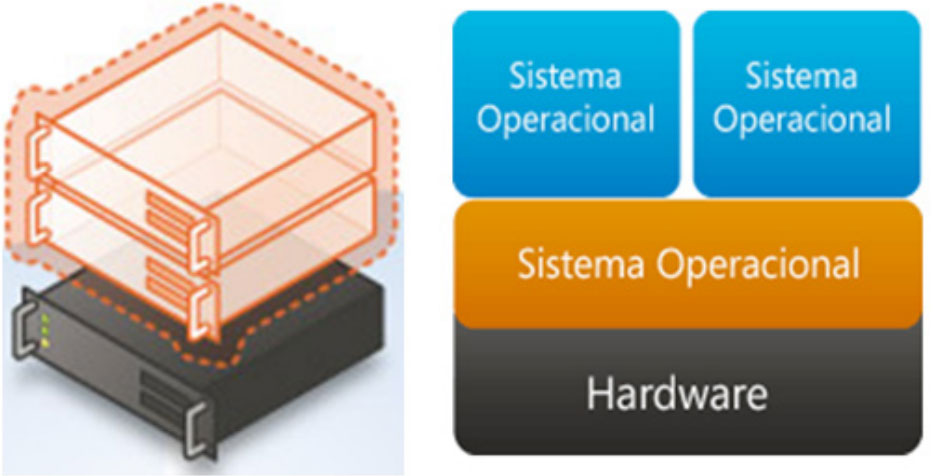
\includegraphics[scale=0.3]{imagens/virtualizacao-servidor.jpg}
    	\end{center}
    	\FonteFigura{\citeonline[p. 163]{neto2015ti}.}
    \end{figure}
    
    \item Virtualização de Estação de Trabalho ou VDI (\textit{Virtual Desktop Infrastructure} - Infraestrutura de estação de trabalho virtual): é utilizado para simular uma maquina virtual "inteira", permitindo o gerenciamento de estações de trabalho com maior eficiência atendendo as necessidades dos usuários. É utilizada para quando existe a necessidade de executar \textit{software} legado\footnote{Termo utilizado para sistemas computacionais que, apesar de serem bastante antigos, fornecem serviços essenciais.}, criar ambientes de testes e treinamento. Cada estação possui seu ambiente com sistema operacional e aplicações independentes. (\autoref{fig_vdi});
    
    \begin{figure}[htb]
    	\caption{\label{fig_vdi}Virtualização de Desktop.}
    	\begin{center}
    	    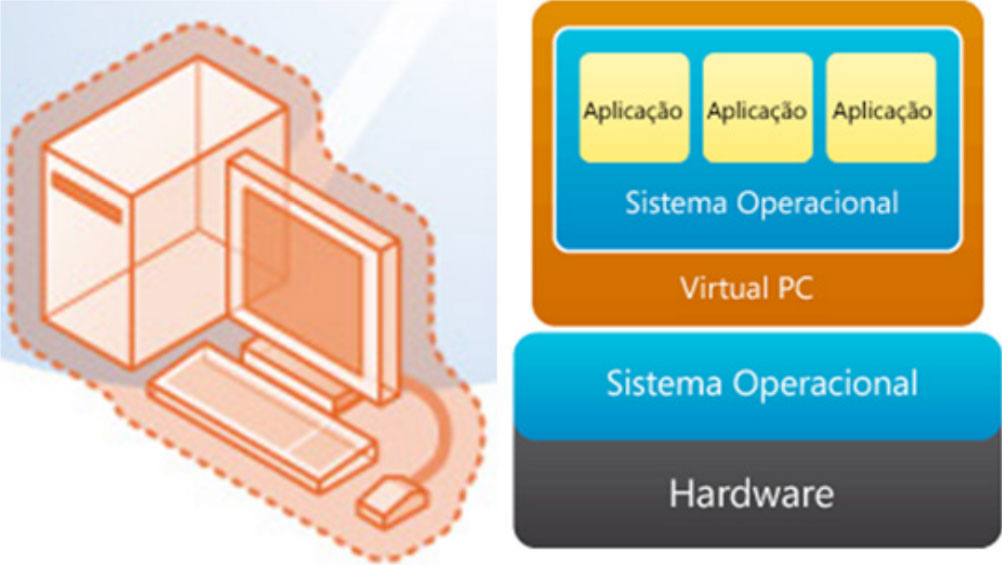
\includegraphics[scale=0.3]{imagens/vdi.jpg}
    	\end{center}
    	\FonteFigura{\citeonline[p. 164]{neto2015ti}.}
    \end{figure}
    
    \item Virtualização de Aplicações: tem como objetivo oferecer aplicações por demanda. A aplicação é alocada em um servidor virtual, que a executa dentro de um próprio ambiente, com isso o usuário não precisa instala-la em sua estação. Cada aplicação fica isolada umas das outras e do sistema operacional subjacente, permitindo ou não a interação e compartilhamento de componentes como dll's\footnote{sigla para \textit{Dynamic Link Library} e se trata de uma biblioteca dinâmica que contém dados que podem ser acessados por mais de um programa instalado no computador} e \textit{Drivers} (\autoref{fig_virt_apli});
    
    \begin{figure}[htb]
    	\caption{\label{fig_virt_apli}Virtualização de Aplicações.}
    	\begin{center}
    	    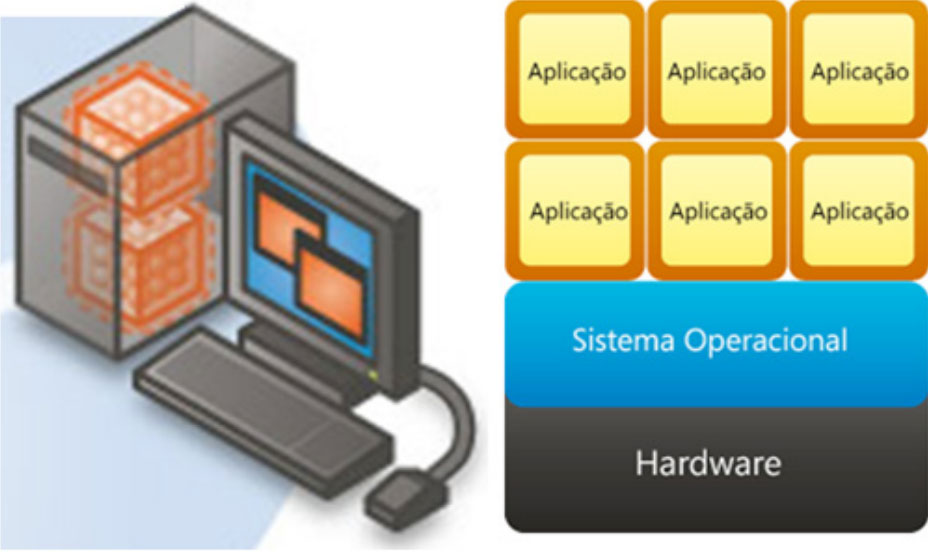
\includegraphics[scale=0.3]{imagens/virtualizacao-aplicacao.jpg}
    	\end{center}
    	\FonteFigura{\citeonline[p. 164]{neto2015ti}.}
    \end{figure} 
    
    \item Virtualização de Apresentação: consiste de um ambiente computacional para acesso à distância, permitindo que uma determinada aplicação seja executada em uma máquina, mas utilize recursos gráficos e de Entrada/Saída de outra e que vários usuários utilizem o sistema não interferindo uns com os outros (\autoref{fig_virt_apre});
    
    \begin{figure}[htb]
    	\caption{\label{fig_virt_apre}Virtualização de Apresentação.}
    	\begin{center}
    	    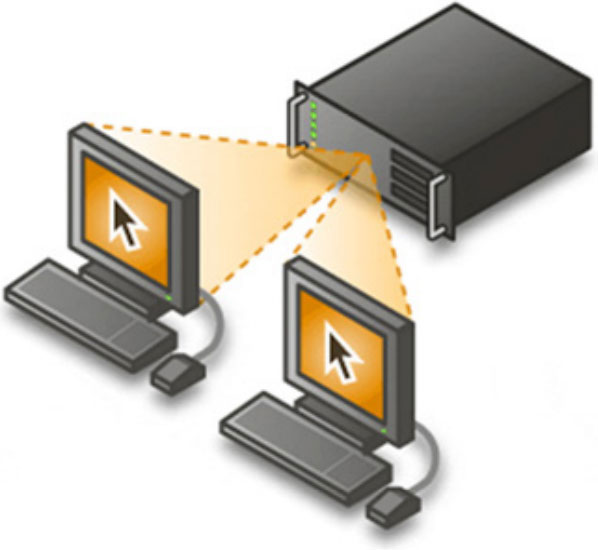
\includegraphics[scale=0.3]{imagens/virtualizacao-apresentacao.jpg}
    	\end{center}
    	\FonteFigura{\citeonline[p. 165]{neto2015ti}.}
    \end{figure}
    
    \item Virtualização de Armazenamento: cria uma camada de abstração entre o sistema operacional e os discos físicos utilizados para armazenamento de dados, permitindo que usuários ou aplicações acessem sem necessidade de informar onde estão localizados ou como é gerenciado (\autoref{fig_virt_arm}).
    
    \begin{figure}[htb]
    	\caption{\label{fig_virt_arm}Virtualização de Armazenamento.}
    	\begin{center}
    	    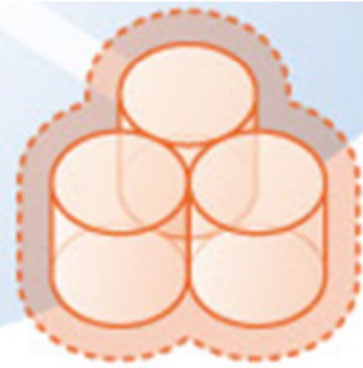
\includegraphics[scale=0.3]{imagens/virtualizacao-armazenamento.jpg}
    	\end{center}
    	\FonteFigura{\citeonline[p. 163]{neto2015ti}.}
    \end{figure}
\end{itemize}

\subsection{Gerenciamento Eletrônico de Documentos}

    
\lipsum[1]
\lipsum[2]
\lipsum[3]

\subsection{Resíduos de Equipamentos Eletroeletrônicos}

Resíduos de Equipamentos Eletroeletrônicos (REEE) é o nome dado a todo resíduo proveniente dos equipamentos eletrônicos \cite[p. 2]{natume2011residuos}. A maioria absoluta desse tipo de resíduo é resultado da obsolescência dos equipamentos eletrônicos, que leva a um descarte de equipamentos antes que esses atinjam seu tempo útil \cite[p. 2]{da2010lixo}. A grande produção de novos aparelhos faz com que os antigos sejam considerados ultrapassados e logo são descartados pelos usuários. Muitas vezes esse descarte é feito de forma inadequada, acarretando assim graves problemas ao meio ambiente.

A \autoref{tab:composicao_fisica} mostra a porcentagem dos principais materiais presentes na composição de um computador, onde eles se encontram e as respectivas porcentagens recicláveis.

\begin{table}[htb]	
    \ABNTEXfontereduzida
	\Caption{\label{tab:composicao_fisica} Composição Física de um computador e índice de materiais recicláveis.}
	\UECEtab{}{
		\begin{tabular}{lp{2.6cm}ll}
			\toprule
    		\textbf{Material} & \textbf{\% em relação ao Peso Total}  & \textbf{\% Reciclável}  & \textbf{Localização} \\
			\midrule \midrule
				Alumínio & 14,172 & 80 & Circuito integrado, solda, bateria \\
				%\midrule
				Chumbo & 6,298 & 5 & Semicondutor \\
				%\midrule
				Ferro & 20,471 & 80 & Estrutura, encaixes \\
				%\midrule
				Estanho & 1,007 & 70 & Circuito integrado \\
				%\midrule
				Cobre & 6,928 & 90 & Condutivo \\
				%\midrule
				Bário & 0,031 & 0 & Válvula eletrônica \\
				%\midrule
				Níquel & 0,850 & 80 & Estrutura, encaixes \\
				%\midrule
				Zinco & 2,204 & 60 & Bateria \\
				%\midrule
				Berílio & 0,015 & 0 & Condutivo térmico, conectores \\
				%\midrule
				Ouro & 0,016 & 98 & Conexão, condutivo \\
				%\midrule
				Manganês & 0,031 & 0 & Estrutura, encaixes \\
				%\midrule
				Prata & 0,018 & 98 & Condutivo \\
				%\midrule
				Cromo & 0,006 & 0 & Decoração, proteção contra corrosão \\
				%\midrule
				Cádmio & 0,009 & 0 & Bateria, chip, semicondutor, estabilizadores \\
				%\midrule
				Mercúrio & 0,002 & 0 & Baterias, ligamentos, termostatos, sensores \\
				%\midrule
				Sílica & 24,880 & 0 & Vidro \\
			\bottomrule
		\end{tabular}
	}{
		\Fonte{\url{http://www.tec.abinee.org.br/2007/arquivos/s702.pdf}}
    }
\end{table}

%pm esse período ficou bem longo também.
%pm vc tá listando três consequências diferentes, dá até pra usar marcador se quiser. enche linguiça e fica menos desgastante de ler
Quando descartados de forma inadequada, em lixões, tem consequências graves ao meio ambiente, como a contaminação de lençóis freáticos e do solo, e às pessoas que entram em contato com esse tipo de lixo devido aos metais pesados neles presentes e as peças plásticas presentes nesses aparelhos demoram cerca de 150 anos para se decompor no meio ambiente \cite[p. 17]{aguilar2009tecnologia}. 

A \autoref{tab:viloes_eletroeletrônicos} mostra os principais metais usados na composição dos equipamentos eletroeletrônicos e os danos causados em humanos que entram em contato com esses equipamentos. Por isso é necessário que o lixo eletrônico seja descartado de forma correta.

\begin{table}[htb]
    \ABNTEXfontereduzida	
	\Caption{\label{tab:viloes_eletroeletrônicos} Os vilões dos eletroeletrônicos.}
	\UECEtab{}{
		\begin{tabular}{p{2cm}p{3.5cm}p{9cm}}
			\toprule
    		\textbf{Substância} & \textbf{Origem} & \textbf{Efeito} \\
			\midrule \midrule
				Mercúrio & Computador, monitor, televisão de tela plana  & Problemas de estômago, distúrbios renais e neurológicos, alterações genéticas e no metabolismo \\
				%\midrule
				Cádmio & Computador, monitor de tubo e baterias & Agente cancerígeno, afeta o sistema nervoso, provoca dores reumáticas, distúrbios metabólicos e 
				problemas pulmonares \\
				%\midrule
				Zinco & Baterias de celulares e laptops & Provoca vômitos, diarreias e problemas pulmonares \\
				%\midrule
				Manganês & Computador e celular & Anemia, dores abdominais, vômito, seborreia, impotência, tremor nas mãos e perturbações emocionais \\
                %\midrule
                Chumbo & Computador, celular e televisão & Irritabilidade, tremores musculares, lentidão de raciocínio, alucinação, insônia e hiperatividade \\
                %\midrule
                PVC & Usado em fios para isolar corrente & Problemas respiratórios  \\
				%\midrule
				Cloreto de Amônia  & Baterias de celulares e laptops & Acumula-se no organismo e provoca asfixia \\
				%\midrule
				Arsênio & Celulares & Agente cancerígeno, afeta o sistema nervoso e cutâneo \\
			\bottomrule
		\end{tabular}
	}{
		\Fonte{Adaptado de \citeonline{moi2014lixo}.}
    }
\end{table}


A melhor forma de evitar a contaminação dos humanos é diminuir a geração desse tipo de resíduo, com a manutenção adequadas dos equipamentos existentes além de práticas que aumentem sua vida útil, bem como destinar os resíduos inevitavelmente gerados para um local específico e adequado para tratamento. Deve haver uma preocupação na produção desses equipamentos, cuidando para que a matéria prima seja bem aproveitada e que não haja desperdícios, além de evitar a produção de equipamentos defeituosos, que terão que ser descartados posteriormente.

A \autoref{fig_percepcao}\footnote{Construído através do Astah Community \url{http://astah.net/editions/community}} apresenta o ciclo de vida de um computador.

\begin{figure}[htb]
	\caption{\label{fig_percepcao}Percepção do problema por mapa conceitual.}
	\begin{center}
	    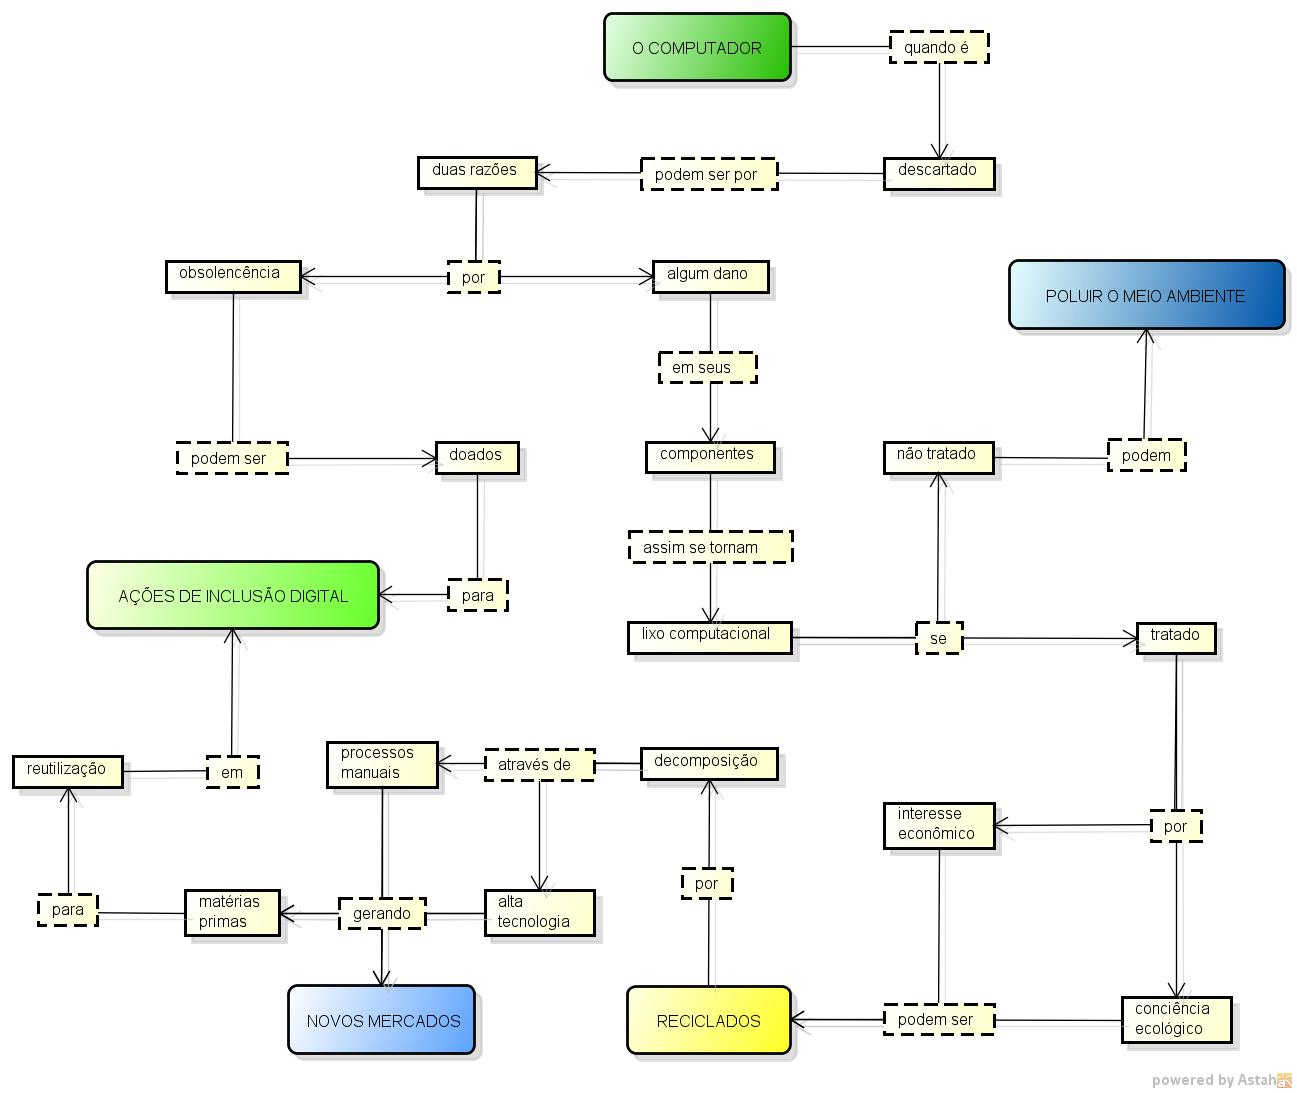
\includegraphics[scale=0.35]{imagens/percepcao-problema.jpg}
	\end{center}
	\Fonte{\citeonline[p. 263]{calvao2009lixo} (Adaptado pelo autor).}
\end{figure}

\subsection{Os cinco R's da educação ambiental}

Os cinco R’s da educação ambiental correspondem a práticas que podem ser implantadas em qualquer lugar e tem impacto que não se limitam ao local em que são aplicados. Sua implantação gera uma economia de recursos elétricas, hídricos e de matéria-prima em geral, além de contribuir para a maior vida útil dos produtos. Como postos nos trabalhos de CITAR os cinco R's podem ser definidos da seguinte forma:

\subsubsection{Repensar}
Antes de adquirir um produto ou serviço deve-se refletir sobre sua real necessidade, ponderando o seu benefício e o impacto ambiental por ele gerado. Além disso deve-se pensar na sua vida útil e em seu posterior descarte, em como ele deve ser feito de forma adequada.

\subsubsection{Recusar}
Caso o produto de interesse não seja de fato necessário, deve-se recusá-lo. Essa prática se aplica a produtos e serviços oferecidos, vide a prática de repensar para decidir sobre sua aceitação ou recusa. Essa prática é muito relevante frente a produtos que contenham materiais que agridam ao meio ambiente e sejam de difícil reciclagem ou demorem para se decompor.

\subsubsection{Reduzir}
Corresponde à redução no consumo de produtos e serviços em geral. Além de reduzir também os gastos que eles geram, desligando aparelhos eletroeletrônicos quando esses não forem usados. Aqui entra também a preferência por produtos de maior durabilidade e que ofereçam menor potencial de geração de resíduos. Isso impacta na redução no número de produtos consumidos e redução nos resíduos gerados.

\subsubsection{Reutilização}
A reutilização corresponde ao uso repetido de um produto, seja para a mesma finalidade sempre, ou dando outra utilidade para ele. Além da troca e doação de produtos para outras pessoas ou empresas.

\subsubsection{Reciclar}
A reciclagem contribui para a economia de recursos usados na produção e no tratamento de resíduos, além de contribuir para a não contaminação de solos e até pessoas pelo descarte inadequado. O ideal é que haja uma separação conforme o tipo de materiais presentes nos resíduos antes da entrega nos postos de coleta seletiva. Essa prática contribui gerando emprego e renda para as pessoas envolvidas, além de resíduos gerados.


\section{Normas, Regulamentações e Certificados}
%pm joga o link do pdf em scholar.google.com
%pm exporta pra bibtex e cola no seu referencias
%pm /cite{nome} e já é
Existem Normas e certificações que servem para regulamentar e atestar as práticas de TI Verde internacional e nacionalmente. Alguns exemplos de certificações internacionais são: ISO 14001, RoHS e Selo Verde, etc. Essas certificações se referem ao processo de trabalho da TI, tanto para a fabricação, quanto para o uso de equipamentos eletrônicos. (Fonte artigo https://assets.itpac.br/arquivos/Revista/42/3.pdf)

\subsection{ISO 14001}
%pm joga o link do pdf em scholar.google.com
%pm exporta pra bibtex e cola no seu referencias
%pm /cite{nome} e já é
A ISO 14001 corresponde a normas que regulamentam os padrões de práticas do trabalho de organizações públicas ou privadas que buscam realizar suas atividades de forma sustentável visando produzir produtos de qualidade que sejam ecologicamente corretos. Fonte artigo https://assets.itpac.br/arquivos/Revista/42/3.pdf

A implantação dessas práticas leva uma revisão dos processos da organização certificada, o que contribui para a redução de poluição, seja pelo lançamentos de gases à atmosfera ou pelos resíduos gerados. 


%A ABNT NBR ISO 14001 é uma norma aceita internacionalmente que define os requisitos para colocar um sistema da gestão ambiental em vigor. Ela ajuda a melhorar o desempenho das empresas por meio da utilização eficiente dos recursos e da redução da quantidade de resíduos, ganhando assim vantagem competitiva e a confiança das partes interessadas.

%A ABNT NBR ISO 14001 adequa-se a todos os tipos e tamanhos da empresa. Ela exige que as empresas considerem todas as questões ambientais relativas às suas operações, como a poluição do ar, questões referentes à água e ao esgoto, a gestão de resíduos, a contaminação do solo, a mitigação e adaptação às alterações climáticas e a utilização e eficiência dos recursos.

%Assim como todas as normas de sistemas da gestão, a ABNT NBR ISO 14001 inclui a necessidade de melhoria contínua dos sistemas de uma empresa e a abordagem de questões ambientais. A norma foi recentemente revista, com melhorias fundamentais, como o aumento da crescente relevância da gestão ambiental nos processos de planejamento estratégico da empresa, maior contribuição por parte da liderança e um compromisso intenso em relação a iniciativas proativas que impulsionem o desempenho ambiental.

%pm usa os marcador certo aqui
%Existem inúmeros motivos para as empresas adotarem uma abordagem estratégica a fim de melhorar o seu desempenho ambiental. Os usuários da norma relataram que a ABNT NBR ISO 14001 ajuda a: • Demonstrar conformidade com requisitos legais e regulamentares atuais e futuros • Aumentar o envolvimento da liderança e o comprometimento dos funcionários • Melhorar a reputação da empresa e a confiança das partes interessadas mediante comunicação estratégica • Alcançar os objetivos estratégicos de negócios através da incorporação de questões ambientais na gestão das empresas. • Oferecer vantagem competitiva e financeira aumentando a eficiência e reduzindo custos • Incentivar a melhoria do desempenho ambiental por parte de fornecedores, integrando-os aos sistemas de negócios da empresa

%A ABNTNBR ISO 14001:2015 passa a exigir: • Que a gestão ambiental seja mais importante no posicionamento estratégico da empresa • Maior comprometimento da liderança • A implementação de iniciativas proativas que visem proteger o meio ambiente contra danos e degradação, como por exemplo, o uso sustentável dos recursos e a mitigação das alterações climáticas • Enfoque no conceito de ciclo de vida a fim de garantir que aspectos ambientais sejam levados em consideração desde o desenvolvimento até o fim da vida útil do produto • A adoção de uma estratégia de comunicação com foco nas partes interessadas Além disso, ela possibilita uma integração mais fácil a outros sistemas de gestão, visto que têm a mesma estrutura e os mesmos termos e definições.
    

\subsection{RoHS}

%pm adiciona isso na lista de siglas, não?
O RoHS (Restriction of Certain Hazardous Substances) ou Restrição de Certas Substâncias Perigosas, também conhecida como a Lei do Sem Chumbo (lead-free), foi criada em julho de 2006 na União Européia. Essa foi uma das primeiras leis a pressionarem as fabricantes de TI. Após a criação da RoHS, as empresas, industrias e importadores também tem o objetivo de se responsabilizar pelo “ciclo de vida” dos produtos que insere no mercado de consumo. Fonte monografia

Entretanto existe uma teoria, do reciclável poluidor, que trata a reciclagem desse REEE como algo tão poluente como o descarte em aterros, bem como a teoria da diminuição do ciclo de vida dos componentes eletrônicos, uma vez que a reciclagem dos componentes pode dar origem a produtos com curta vida útil (Garcia e Milagre, 2008). 

\subsection{WEEE}

A WEEE (Waste Electrical and Electronic Equipment Directive) ou Diretiva para o Lixo Elétrico e Equipamentos Eletrônicos também foi criada na Europa com o objetivo de preservar a natureza, essa diretiva determina como compromisso dos fabricantes o recolhimento e a destinação correta dos resíduos por eles gerados. A WEEE também prevê a reciclagem, recuperação e reutilização dos resíduos para que estes sejam reduzidos \cite{neto2015ti}.

\subsection{Selo Verde}

O selo verde é uma forma de reconhecimento de espaços, produtos e serviços que contribuam para a preservação ambiental. Tal selo é atribuído as organizações depois das organizações passarem por controle de qualidade ambiental. Com isso há o incentivo a promoção de soluções ambientais (Fonte: http://seloverde.org/), uma vez que os critérios utilizados para certificar uma organização são:  a promoção da conscientização ambiental na comunidade que adquire seus produtos ou serviços, ser economicamente viável e promover a sustentabilidade econômica do ambiente digital e ser ambientalmente responsável, aplicando os 5R’s em seus processos de forma a produzir com economia de energia ou com pequena quantidade de substâncias tóxicas. (Fonte: implementacoa de praticas sustentaveis em empresas.pdf). 
É uma forma de incentivar as empresas a fabricarem produtos com baixa quantidade de produtos químicos (Fonte: https://assets.itpac.br/arquivos/Revista/42/3.pdf), além de ser um diferencial no mercado. Alguns dos órgãos responsáveis pela aplicação desses selos são: o Greenpeace, o Centro de Computação Eletrônica da Universidade de São Paulo, Instituto da Qualidade Automotiva e Forset Stewardship Council- FSC.  (Fonte: https://assets.itpac.br/arquivos/Revista/42/3.pdf)


\subsection{Energy Star}

Energy Star e um programa da U.S. Environmental Protection Agency(EPA) que incentiva a redução na quantidade de energia consumida as organizações. Uma de suas práticas é oferecer selos aos fabricantes de equipamentos eletrônicos que optarem pela utilização de tecnologias com funções para poupar energia.

\subsection{Procel}

O Selo Procel de Economia de Energia foi criado pelo Programa Nacional de Conservação de Energia Elétrica – Procel, programa instituído por Decreto Presidencial em 8 de dezembro de 1993, sendo desde então executado pela Eletrobras. O objetivo é criar uma identificação para que o consumidor conheça os equipamentos e eletrodomésticos mais eficientes e que consomem menos energia.

A classificação dos equipamentos é feita de acordo com os índices de consumo e desempenho estabelecidos para cada categoria de equipamento. Para receber o selo cada equipamento é submetido a ensaios em laboratórios indicados pela Eletrobras.


\subsection{Legislação Brasileira}
%pm Lei não é publicação científica.
%pm essas porra vira tudo footnote, com a \url de cada uma e a data de acesso.

Lei nº 12.305 de 2 de agosto de 2010. (projeto de lei 2061/07)

No Brasil, a Lei nº 12.305, de 02 de agosto de 2010, institui a Política Nacional de Resíduos Sólidos, dispõe “sobre seus princípios, objetivos e instrumentos, bem como sobre as diretrizes relativas à gestão integrada e ao gerenciamento de resíduos sólidos, incluídos os perigosos, às responsabilidades dos geradores e do poder público e aos instrumentos econômicos aplicáveis. ” (LEI Nº 12.305, 2010, Art. 1o  § 1º, p. 1).

Alguns princípios e objetivos da Política Nacional de Resíduos Sólidos são: o desenvolvimento sustentável; a ecoeficiência, visando fornecimento de bens e serviços de um melhor custo-benefício e redução de impactos ambientais; a responsabilidade compartilhada pelo ciclo de vida dos produtos; a proteção da saúde pública e da qualidade ambiental; a aplicação de alguns dos 5R’s, bem como o tratamento adequada dos rejeitos. (Lei Nº 12.305, 2010, Art. 6º e 7º)

No que diz respeito a tecnologia da informação, um dos objetivos trata da “adoção, desenvolvimento e aprimoramento de tecnologias limpas como forma de minimizar impactos ambientais (Art. 7o IV).

Uma das diretrizes trata da ordem de prioridade na gestão e gerenciamento de resíduos sólidos: “não geração, redução, reutilização, reciclagem, tratamento dos resíduos sólidos e disposição final ambientalmente adequada dos rejeitos.” (Art. 9o)

Os responsáveis pelo destino dos resíduos de eletrônicos são definidos no Art. 33. São eles os fabricantes, importadores, distribuidores e comerciantes de produtos eletroeletrônicos. Eles tem como obrigação “a estruturar e implementar sistemas de logística reversa, mediante retorno dos produtos após o uso pelo consumidor, de forma independente do serviço público de limpeza urbana e de manejo dos resíduos sólidos”. Além disso devem “tomar todas as medidas necessárias para assegurar a implementação e operacionalização do sistema de logística reversa sob seu encargo [...], podendo, [...] implantar procedimentos de compra de produtos ou embalagens usados; disponibilizar postos de entrega de resíduos reutilizáveis e recicláveis; atuar em parceria com cooperativas ou outras formas de associação de catadores de materiais reutilizáveis e recicláveis” (Art. 33. § 3o I, II e III).

O Art. 5o diz que a “Política Nacional de Resíduos Sólidos integra a Política Nacional do Meio Ambiente e articula-se com a Política Nacional de Educação Ambiental, regulada pela Lei no 9.795, de 27 de abril de 1999, com a Política Federal de Saneamento Básico, regulada pela Lei nº 11.445, de 2007. Além delas se aplica também aos resíduos sólidos a lei nos 11.445, de 5 de janeiro de 2007, dentre outras normas (Art. 2o).

Política Nacional de Educação Ambiental (Lei nº 9.785 de 27 de abril de 1999). 

Nessa lei a educação ambiental é tratada como “os processos por meio dos quais o indivíduo e a coletividade constroem valores sociais, conhecimentos, habilidades, atitudes e competências voltadas para a conservação do meio ambiente, bem de uso comum do povo, essencial à sadia qualidade de vida e sua sustentabilidade. (Art. 1o)

Segunda Art. 2o da Lei, cabe às empresas, entidades de classe, instituições públicas e privadas, a promoção de “programas destinados à capacitação dos trabalhadores, visando à melhoria e ao controle efetivo sobre o ambiente de trabalho, bem como sobre as repercussões do processo produtivo no meio ambiente”. Além disso, empresas públicas e privadas devem ser incentivadas, pelo Poder Público, em níveis federal, estadual e municipal, a participarem do desenvolvimento de programas de educação ambiental (Art. 13. Parágrafo único III) não formal, que tem por objetivo sensibilizar a população em geral sobre as questões ambientais e à sua organização e participação na defesa da qualidade do meio ambiente. (Art. 13.)

Política Federal de Saneamento Básico (Lei nº 11.445 de 2007)

Um dos princípios fundamentais dessa lei é a “utilização de tecnologias apropriadas [...] e a adoção de soluções graduais e progressivas (Art. 2o  VIII) e uma das diretrizes incentiva o “desenvolvimento científico e tecnológico, à adoção de tecnologias apropriadas e à difusão dos conhecimentos gerados” (Art. 48. VIII). Essa lei também estimula o “uso de tecnologias modernas e eficientes, compatíveis com os níveis exigidos de qualidade, continuidade e segurança na prestação dos serviços” (Art. 29.  § 1o  VII).

% ----------------------------------------------------------
% PARTE III
% ----------------------------------------------------------
\part{Levantamento Amostral}


\chapter{Estudo de caso}\label{chap:estudodecaso}

\section{Universidade Estadual do Sudoeste da Bahia}

A Universidade Estadual do Sudoeste da Bahia está situada na Mesorregião do Centro-Sul Baiano, que é formada pela união de 118 municípios, com 2.478.542 habitantes em uma área de 127.878 km$^{2}$, o que corresponde aproximadamente 22,7\% de todo o território da Bahia.$^{[}$\footnote{Informações retiradas do site Cidade Brasil, Disponível em: \url{https://www.cidade-brasil.com.br/mesorregiao-do-centro-sul-baiano.html}. Acessado em 16 de junho de 2018}$^{]}$ Ela é constituída de três campi, Vitória da Conquista, Jequié e Itapetinga, tendo sede em Vitória da Conquista, local em que foi realizado o estudo de caso, e à 510 km da capital Salvador. O município de Vitória da Conquista conta com um território de 3.705,838 km$^{2}$ e uma população com 348.718 habitantes.$^{[}$\footnote{Informações retiradas do site Cidades IBGE, Disponível em: \url{https://cidades.ibge.gov.br/brasil/ba/vitoria-da-conquista}.  Acessado em 16 de junho de 2018}$^{]}$

A UESB, campus de Vitória da Conquista, tornou-se o campo desta pesquisa, pois a mesma é uma ampla consumidora e usuária de equipamentos tecnológicos, possuindo um conjunto de equipamentos, computadores, \textit{switches}, servidores, pontos de acessos para rede sem fio, entre outros dispositivos de informática. Segundo o Roteiro de Diagnóstico Setorial$^{[}$\footnote{Roteiro de Diagnóstico Setorial, Disponível em: \url{http://www2.uesb.br/wp-content/uploads/2018/05/UINFOR.pdf}.  Acessado em 16 de junho de 2018}$^{]}$ a UESB possui atualmente nos três campi aproximadamente 2500 computadores, incluindo notebooks, sendo em sua maioria equipamentos antigos. Diante disso, existe uma necessidade de se verificar e propor meios para que se tenha uma diminuição dos riscos ou dos impactos ambientais causados pela má utilização da tecnologia, servindo de exemplo para a comunidade.

A Unidade Organizacional de Informática (UINFOR) foi escolhida para ser o foco desta pesquisa, pois a mesma é responsável pela gestão da TI na UESB, sendo então a principal encarregada de implementar práticas que busquem a sustentabilidade na utilização da TI. 

\subsection{Unidade Organizacional de Informática}

A UINFOR é um órgão de assessoria da reitoria na gestão da Tecnologia da Informação e Comunicação (TIC). As TIC's são fundamentais para o bom funcionamento da Universidade nas áreas administrativas e nas acadêmicas (ensino, pesquisa e extensão). 

Algumas estratégias adotadas são: Prioridade para uso do software livre para redução de custos; uso de serviços gratuitos de computação em nuvem; busca de financiamento de outras formas de sustentação para a expansão da conectividade da internet e dos sistemas; e trabalhar em parceria com a Assessoria na Gestão de Projetos e Convênios Institucionais (AGESPI) em projetos (emendas parlamentares e outras formas) para o financiamento da infraestrutura computacional.

A UINFOR possui atualmente os seguintes setores que são ilustrados na \autoref{fig_organograma}:

\begin{figure}[htb]
    \caption{\label{fig_organograma}Organograma da UINFOR.}
    \begin{center}
        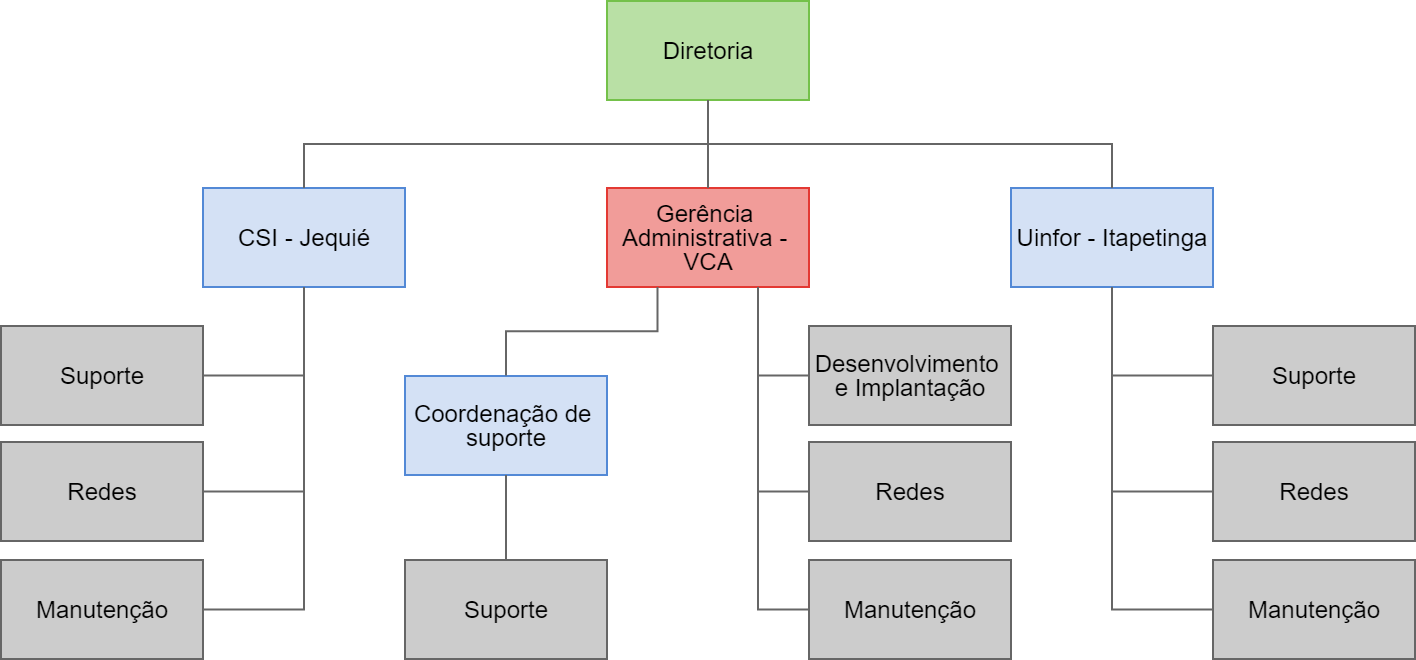
\includegraphics[scale=0.32]{imagens/organograma.png}
    \end{center}
    \FonteFigura{Roteiro de Diagnóstico Setorial.}
\end{figure}

\begin{itemize}
    \item Manutenção: realiza atividades como formatação e instalação de sistemas operacionais e outros softwares, troca de peças defeituosas, concerto de equipamentos com problemas, entre outras atividades relacionada aos equipamentos de informática.
    \item Redes: responsável por serviços de configuração da rede sem fio e com fio, implementação do cabeamento estruturado, configuração dos equipamentos de rede como roteadores, \textit{switches} e pontos de acesso sem fio. No campos de Vitória da Conquista o setor executa algumas atividades mais avançadas, como o gerenciamento da infra estrutura do \textit{datacenter} da UESB. 
    \item Suporte: atua no suporte ao uso dos sistemas de informação da universidade.
    \item Coordenação de suporte: responsável pelo relacionamento técnico com as empresas dos sistemas SAGRES e Pergamum e com o programa Mais Futuro.
    \item Gerencia Administrativa do campus de Vitória da Conquista: auxilia nos processos administrativos em geral, gerenciamento de pessoal, atendimento ao público, controle dos contratos gerenciados pela UINFOR, entre outros.
    \item Diretoria: encarregado das atividades como: assessorar a reitoria na gestão das TIC's; coordenar as áreas operacionais dos três campi; realizar o planejamento de aquisição de equipamentos e serviços de TIC's; emitir pareceres técnicos para subsidiar decisões da procuradoria jurídica e dos setores de licitações; e elaborar projetos juntamente com a AGESPI que visam financiar as TIC's.
\end{itemize}

\section{Avaliação da aplicação da TI Verde na UESB}

Foi realizada uma entrevista e a aplicação de um questionário com o diretor da UINFOR. A entrevista foi realizada no dia 15 de Junho de 2018, utilizando o aplicativo de mensagens instantâneas \textit{WhatsApp Messenger}, já o questionário foi aplicado no dia 17 de Abril de 2018, utilizando o editor de texto online Google Documentos. Também foi realizado a leitura do Roteiro de Diagnóstico Setorial, disponibilizado pelo entrevistado, que descreve todas as funções, atribuições, atividades, estruturas e processos da UINFOR, além do Plano de Desenvolvimento Institucional 2013-2017$^{[}$\footnote{PID 2013-2017, Disponível em: \url{http://www.uesb.br/pdi/arquivos/PDI_Final.pdf}.  Acessado em 16 de junho de 2018}$^{]}$ que contém diversas informações sobre a UESB.

O questionário aplicado foi extraído de \citeonline{lunardi2014desenvolvimento}, e serve para avaliar o grau de utilização da TI Verde pelas organizações. Ele é dividido em 5 fatores, apresentados a seguir: 
\begin{itemize}
    \item  \textbf{Consciência socioambiental:} Avalia se a organização está consciente da necessidade de abordar as questões ambientas de forma mais proativa;
    \item \textbf{Ações sustentáveis:} Avalia se a organização implementa iniciativas para tornar os processos o mais sustentável possível;
    \item \textbf{\textit{Expertise} ambiental:} Avalia se a organização se submete a experimentar, atualizar e buscar novas abordagens, informações e conhecimentos a fim de aplicar estratégias sustentáveis na área de TI;
    \item \textbf{Monitoramento:} Avalia se a organização gerencia as atividades e medidas de TI voltadas à redução do consumo de recursos e dos danos ao meio ambiente;
    \item \textbf{Orientação ambiental:} Avalia se a organização está comprometida com a sustentabilidade e com o suporte às inovações ambientais.
\end{itemize}

Com a aplicação do questionário, foi constatado que os seguintes fatores estão abaixo da média apresentada por \citeonline{lunardi2014desenvolvimento}: 
\begin{itemize}
    \item \textbf{Consciência socioambiental:} Existe falta de estratégias e políticas ambientais e para a utilização de recursos naturais como água, luz e papel. Apesar de frequentemente procurar parceiros comerciais que têm preocupações ambientais, a UESB só em algumas vezes pode ser considerada ambientalmente sustentável; 
    \item \textbf{Monitoramento:} Frequentemente controla os custos com manutenção dos equipamentos computacionais, mas em poucas ocasiões faz o gerenciamento do consumo de energia e o desempenho do mesmo;
    \item \textbf{Orientação ambiental:} Embora frequentemente incentive a reciclagem e faça recomendações aos funcionários de como economizar os produtos computacionais, falta uma preocupação com a conscientização dos funcionários, para que os mesmos apaguem a luz, utilizem o modo de descanso e desliguem os comutadores quando não estão em uso.
\end{itemize}

Já os seguintes fatores estão na média ou acima dela:

\begin{itemize}
    \item \textbf{\textit{Expertise} ambiental:} Foi verificado que a UINFOR possui um grande conhecimento sobre como diferentes tecnologias computacionais podem funcionar de forma mais eficiente e quais estão disponíveis no mercado. Ela também recorre a diferentes fontes para identificar tendencias mais limpas e econômicas e busca novas formas de redução do consumo de energia dos produtos computacionais como computadores, servidores e \textit{datacenters}. Em contrapartida, novamente foi verificado a falta de conscientização dos funcionários, sobre o uso racional dos recursos computacionais. 
    \item \textbf{Ações sustentáveis:} Fator em que a UINFOR mais se destaca, aplicando diferentes estratégias para melhor utilização dos produtos computacionais, removendo equipamentos computacionais que não estão em uso e fazendo suas últimas aquisições tecnológicas levando em consideração a eficiência energética. O único ponto abaixo foi o fato de como a grande maioria dos computadores da UESB foram adquiridos anos atrás, eles atualmente não são eficientes em termos de energia.
\end{itemize}

Com base na análise da entrevista realizada, do questionário aplicado e dos documentos lidos, pode-se compreender alguns pontos importantes para a pesquisa. Atualmente a UINFOR/UESB não possui estratégias e políticas ambientais bem definidas, embora utilize algumas práticas sustentáveis, que na maioria das vezes são utilizadas visando à economia e redução de gastos, se encaixando no primeiro nível das práticas da TI Verde, o TI Verde Tático. A seguir estes pontos são apresentados. 

A coleta, armazenamento e descarte dos REEE são realizadas da seguinte forma: Quando algum departamento detecta qualquer problema em algum equipamento eletroeletrônico, é aberto um chamado e o setor de manutenção realiza a busca do equipamento, os resíduos gerados pela manutenção são encaminhados para o almoxarifado, de lá os resíduos são enviados para uma central em Salvador, está central que realiza o processo de descarte, mas este processo é desconhecido pela UINFOR.

Na hora da aquisição de novos equipamentos, os selos Energy Star e RoHS são exigidos nas licitações realizadas. A equipe não possuí o conhecimentos dos 5 R's da sustentabilidade, embora seja levada a reduzir e reutilizar por conta da falta de verba.

Na opinião do diretor da UINFOR, a UESB precisa de estratégias para o consumo de água e de energia, além da utilização de um sistema de energia de 48 \textit{volts} para o \textit{datacenter} e a utilização de Computadores de Placa Única, para melhorar a sua sustentabilidade ambiental.

As principais práticas de TI Verde que a UINFOR utiliza são a Virtualização e o Gerenciamento Eletrônico de Documentos, explicadas a seguir.

A Virtualização tem como benefício a economia de gastos com hardware e a otimização do parque de servidores. Ela é utilizada para o compartilhamento de dezenas de servidores físicos, facilitando a administração e a otimização dos recursos. Ela é feita através do uso do programa \textit{VMware}. 

Já quanto ao Gerenciamento Eletrônico de Documentos, foi identificado que até então a UESB utilizava o sistema Lúpus, desenvolvido pela própria UESB. O Lúpus era responsável pela tramitação dos processos da UESB, mas ele está sendo descontinuado e sendo migrado para o Sistema Eletrônico de Informação (SEI). Outra aplicação é através do projeto de Gestão Eletrônica de Documentos (GED).

\subsection{Projeto de Gestão Eletrônica de Documentos}

Para um melhor entendimento e compreensão do projeto, foi realizada uma entrevista com o analista e desenvolvedor do projeto no dia 14 de junho de 2014, utilizando o editor de texto online Google Documentos.

O projeto de GED tem como piloto o setor de Recursos Humanos (RH), é implementado através da modificação do software livre Alfresco, são utilizadas técnicas e padrões para recebimento, preparação, digitalização, indexação em software e disponibilização do acesso aos documentos por um meio digital. Ele tem como objetivos centralizar as fontes de informação da UESB, aumentar a acessibilidade à informação e armazenar os arquivos físicos de forma adequada.

A principal motivação do projeto piloto de GED, na área de RH, foi a opinião da equipe do setor, demonstrada através de uma consulta interna, indicando os prontuários físicos como a fonte mais confiável de informações. Através deste levantamento, foi decidido o investimento na digitalização e disponibilização dos documentos via ferramenta de software.

O projeto foi idealizado em 2011, inicialmente, buscando a terceirização da demanda. A partir de 2013, o Setor de Informações Funcionais (SIF/RH) assumiu a implantação do projeto. Atualmente ele está funcionando na Assessoria de Gestão de Pessoas (APG) e no Posto de Cadastro de Fornecedores (PCF), e se encontra em fase de análise/implantação na Reitoria e no Centro Universitário de Atenção à Saúde (CEUAS). 

O projeto tem caráter de aplicação contínua, e é esperado um processo maduro de produção e/ou recepção de documentos, armazenamento, descarte e acesso eficiente às informações. Entre as principais conquistas, estão a formação de uma equipe com conhecimento na área de GED, o crescente reconhecimento por parte da UESB e uma base de dados/documentos cada vez mais robusta. 

O estado atual do projeto pode ser classificado como "híbrido", pelo fato de ainda se trabalhar com documentos tanto em papel como em meio digital. A maior parte dos documentos que já foram digitalizados são recebidos mensalmente pelo GED-RH. Mas, além destes, existem documentos que já existiam antes do início do projeto, que ainda não foram processados, o que depende de mais pessoal, equipamentos e espaço para ser feito.

\subsection{Sistema Eletrônico de Informação}

O SEI foi desenvolvido pelo Tribunal Regional Federal da 4ª Região (TRF4), sendo um sistema de gestão de processos e documentos arquivísticos eletrônicos. As principais características são a libertação do papel como suporte físico para documentos institucionais e o compartilhamento do conhecimento com atualização e comunicação de novos eventos em tempo real. Ele faz parte de uma iniciativa conjunta de órgãos e entidades de diversas esferas da Administração Pública, sendo um produto do projeto Processo Eletrônico Nacional (PEN), possibilitando melhorias como ganhos em agilidade, produtividade, transparência e satisfação do público usuário, além de uma redução de custos. Ele permite a produção, edição, assinatura e trâmite de documentos, suas principais facilidades são: Portabilidade; Acesso Remoto; Acesso de usuários externos; Controle de nível de acesso; Tramitação em múltiplas unidades; Funcionalidades específicas; e Sistema intuitivo.$^{[}$\footnote{Informações retiradas do Manual do Usuário SEI, Disponível em: \url{https://softwarepublico.gov.br/social/articles/0004/9746/sei-doc-usuario.pdf}.  Acessado em 24 de junho de 2018}$^{]}$

Segundo uma matéria divulgada pelo portal do SEI Bahia$^{[}$\footnote{SEI Bahia já gerou economia de 7,5 milhões de folhas de papel, Disponível em: \url{http://www.portalseibahia.saeb.ba.gov.br/noticias/2018-06-15/sei-bahia-ja-gerou-economia-de-75-milhoes-de-folhas-de-papel}.  Acessado em 24 de junho de 2018}$^{]}$ o governo baiano já deixou de consumir 7,5 milhões de folhas de papel desde a implantação do projeto, e segundo o secretário de Administração do Estado, Edelvido Góes, a partir do dia 1º de novembro de 2018, todos os processos do Estado deverão tramitar obrigatoriamente em meio eletrônico através do sistema. O sistema já se encontra em fase de implantação e treinamento na UESB.

\section{Propostas}

\lipsum[3]

% ----------------------------------------------------------
% PARTE III
% ----------------------------------------------------------
%\part{Conclusão}

%%% abtex2-modelo-include-comandos.tex, v-1.9.2 laurocesar
%% Copyright 2012-2014 by abnTeX2 group at http://abntex2.googlecode.com/ 
%%
%% This work may be distributed and/or modified under the
%% conditions of the LaTeX Project Public License, either version 1.3
%% of this license or (at your option) any later version.
%% The latest version of this license is in
%%   http://www.latex-project.org/lppl.txt
%% and version 1.3 or later is part of all distributions of LaTeX
%% version 2005/12/01 or later.
%%
%% This work has the LPPL maintenance status `maintained'.
%% 
%% The Current Maintainer of this work is the abnTeX2 team, led
%% by Lauro César Araujo. Further information are available on 
%% http://abntex2.googlecode.com/
%%
%% This work consists of the files abntex2-modelo-include-comandos.tex
%% and abntex2-modelo-img-marca.pdf
%%

% ---
% Este capítulo, utilizado por diferentes exemplos do abnTeX2, ilustra o uso de
% comandos do abnTeX2 e de LaTeX.
% ---
 
\chapter{Resultados de comandos}\label{cap_exemplos}

\chapterprecis{Isto é uma sinopse de capítulo. A ABNT não traz nenhuma
normatização a respeito desse tipo de resumo, que é mais comum em romances 
e livros técnicos.}\index{sinopse de capítulo}

% ---
\section{Codificação dos arquivos: UTF8}
% ---

A codificação de todos os arquivos do \abnTeX\ é \texttt{UTF8}. É necessário que
você utilize a mesma codificação nos documentos que escrever, inclusive nos
arquivos de base bibliográficas |.bib|.

% ---
\section{Citações diretas}
\label{sec-citacao}
% ---

\index{citações!diretas}Utilize o ambiente \texttt{citacao} para incluir
citações diretas com mais de três linhas:

\begin{citacao}
As citações diretas, no texto, com mais de três linhas, devem ser
destacadas com recuo de 4 cm da margem esquerda, com letra menor que a do texto
utilizado e sem as aspas. No caso de documentos datilografados, deve-se
observar apenas o recuo \cite[5.3]{NBR10520:2002}.
\end{citacao}

Use o ambiente assim:

\begin{verbatim}
\begin{citacao}
As citações diretas, no texto, com mais de três linhas [...] deve-se observar
apenas o recuo \cite[5.3]{NBR10520:2002}.
\end{citacao}
\end{verbatim}

O ambiente \texttt{citacao} pode receber como parâmetro opcional um nome de
idioma previamente carregado nas opções da classe (\autoref{sec-hifenizacao}). Nesse
caso, o texto da citação é automaticamente escrito em itálico e a hifenização é
ajustada para o idioma selecionado na opção do ambiente. Por exemplo:

\begin{verbatim}
\begin{citacao}[english]
Text in English language in italic with correct hyphenation.
\end{citacao}
\end{verbatim}

Tem como resultado:

\begin{citacao}[english]
Text in English language in italic with correct hyphenation.
\end{citacao}

\index{citações!simples}Citações simples, com até três linhas, devem ser
incluídas com aspas. Observe que em \LaTeX as aspas iniciais são diferentes das
finais: ``Amor é fogo que arde sem se ver''.

% ---
\section{Notas de rodapé}
% ---

As notas de rodapé são detalhadas pela NBR 14724:2011 na seção 5.2.1\footnote{As
notas devem ser digitadas ou datilografadas dentro das margens, ficando
separadas do texto por um espaço simples de entre as linhas e por filete de 5
cm, a partir da margem esquerda. Devem ser alinhadas, a partir da segunda linha
da mesma nota, abaixo da primeira letra da primeira palavra, de forma a destacar
o expoente, sem espaço entre elas e com fonte menor
\citeonline[5.2.1]{NBR14724:2011}.}\footnote{Caso uma série de notas sejam
criadas sequencialmente, o \abnTeX\ instrui o \LaTeX\ para que uma vírgula seja
colocada após cada número do expoente que indica a nota de rodapé no corpo do
texto.}\footnote{Verifique se os números do expoente possuem uma vírgula para
dividi-los no corpo do texto.}. 


% ---
\section{Tabelas}
% ---

\index{tabelas}A \autoref{tab-nivinv} é um exemplo de tabela construída em
\LaTeX.

\begin{table}[htb]
\ABNTEXfontereduzida
\caption[Níveis de investigação]{Níveis de investigação.}
\label{tab-nivinv}
\begin{tabular}{p{2.6cm}|p{6.0cm}|p{2.25cm}|p{3.40cm}}
  %\hline
   \textbf{Nível de Investigação} & \textbf{Insumos}  & \textbf{Sistemas de Investigação}  & \textbf{Produtos}  \\
    \hline
    Meta-nível & Filosofia\index{filosofia} da Ciência  & Epistemologia &
    Paradigma  \\
    \hline
    Nível do objeto & Paradigmas do metanível e evidências do nível inferior &
    Ciência  & Teorias e modelos \\
    \hline
    Nível inferior & Modelos e métodos do nível do objeto e problemas do nível inferior & Prática & Solução de problemas  \\
   % \hline
\end{tabular}
\legend{Fonte: \citeonline{van86}}
\end{table}

Já a \autoref{tabela-ibge} apresenta uma tabela criada conforme o padrão do
\citeonline{ibge1993} requerido pelas normas da ABNT para documentos técnicos e
acadêmicos.

\begin{table}[htb]
\IBGEtab{%
  \caption{Um Exemplo de tabela alinhada que pode ser longa
  ou curta, conforme padrão IBGE.}%
  \label{tabela-ibge}
}{%
  \begin{tabular}{ccc}
  \toprule
   Nome & Nascimento & Documento \\
  \midrule \midrule
   Maria da Silva & 11/11/1111 & 111.111.111-11 \\
  \midrule 
   João Souza & 11/11/2111 & 211.111.111-11 \\
  \midrule 
   Laura Vicuña & 05/04/1891 & 3111.111.111-11 \\
  \bottomrule
\end{tabular}%
}{%
  \fonte{Produzido pelos autores.}%
  \nota{Esta é uma nota, que diz que os dados são baseados na
  regressão linear.}%
  \nota[Anotações]{Uma anotação adicional, que pode ser seguida de várias
  outras.}%
  }
\end{table}


% ---
\section{Figuras}
% ---

\index{figuras}Figuras podem ser criadas diretamente em \LaTeX,
como o exemplo da \autoref{fig_circulo}.

\begin{figure}[htb]
	\caption{\label{fig_circulo}A delimitação do espaço}
	\begin{center}
	    \setlength{\unitlength}{5cm}
		\begin{picture}(1,1)
		\put(0,0){\line(0,1){1}}
		\put(0,0){\line(1,0){1}}
		\put(0,0){\line(1,1){1}}
		\put(0,0){\line(1,2){.5}}
		\put(0,0){\line(1,3){.3333}}
		\put(0,0){\line(1,4){.25}}
		\put(0,0){\line(1,5){.2}}
		\put(0,0){\line(1,6){.1667}}
		\put(0,0){\line(2,1){1}}
		\put(0,0){\line(2,3){.6667}}
		\put(0,0){\line(2,5){.4}}
		\put(0,0){\line(3,1){1}}
		\put(0,0){\line(3,2){1}}
		\put(0,0){\line(3,4){.75}}
		\put(0,0){\line(3,5){.6}}
		\put(0,0){\line(4,1){1}}
		\put(0,0){\line(4,3){1}}
		\put(0,0){\line(4,5){.8}}
		\put(0,0){\line(5,1){1}}
		\put(0,0){\line(5,2){1}}
		\put(0,0){\line(5,3){1}}
		\put(0,0){\line(5,4){1}}
		\put(0,0){\line(5,6){.8333}}
		\put(0,0){\line(6,1){1}}
		\put(0,0){\line(6,5){1}}
		\end{picture}
	\end{center}
	\legend{Fonte: os autores}
\end{figure}

Ou então figuras podem ser incorporadas de arquivos externos, como é o caso da
\autoref{fig_grafico}. Se a figura que ser incluída se tratar de um diagrama, um
gráfico ou uma ilustração que você mesmo produza, priorize o uso de imagens
vetoriais no formato PDF. Com isso, o tamanho do arquivo final do trabalho será
menor, e as imagens terão uma apresentação melhor, principalmente quando
impressas, uma vez que imagens vetorias são perfeitamente escaláveis para
qualquer dimensão. Nesse caso, se for utilizar o Microsoft Excel para produzir
gráficos, ou o Microsoft Word para produzir ilustrações, exporte-os como PDF e
os incorpore ao documento conforme o exemplo abaixo. No entanto, para manter a
coerência no uso de software livre (já que você está usando \LaTeX e \abnTeX),
teste a ferramenta \textsf{InkScape}\index{InkScape}
(\url{http://inkscape.org/}). Ela é uma excelente opção de código-livre para
produzir ilustrações vetoriais, similar ao CorelDraw\index{CorelDraw} ou ao Adobe
Illustrator\index{Adobe Illustrator}. De todo modo, caso não seja possível
utilizar arquivos de imagens como PDF, utilize qualquer outro formato, como
JPEG, GIF, BMP, etc. Nesse caso, você pode tentar aprimorar as imagens
incorporadas com o software livre \textsf{Gimp}\index{Gimp}
(\url{http://www.gimp.org/}). Ele é uma alternativa livre ao Adobe
Photoshop\index{Adobe Photoshop}.

\begin{figure}[htb]
	\caption{\label{fig_grafico}Gráfico produzido em Excel e salvo como PDF}
	\begin{center}
	    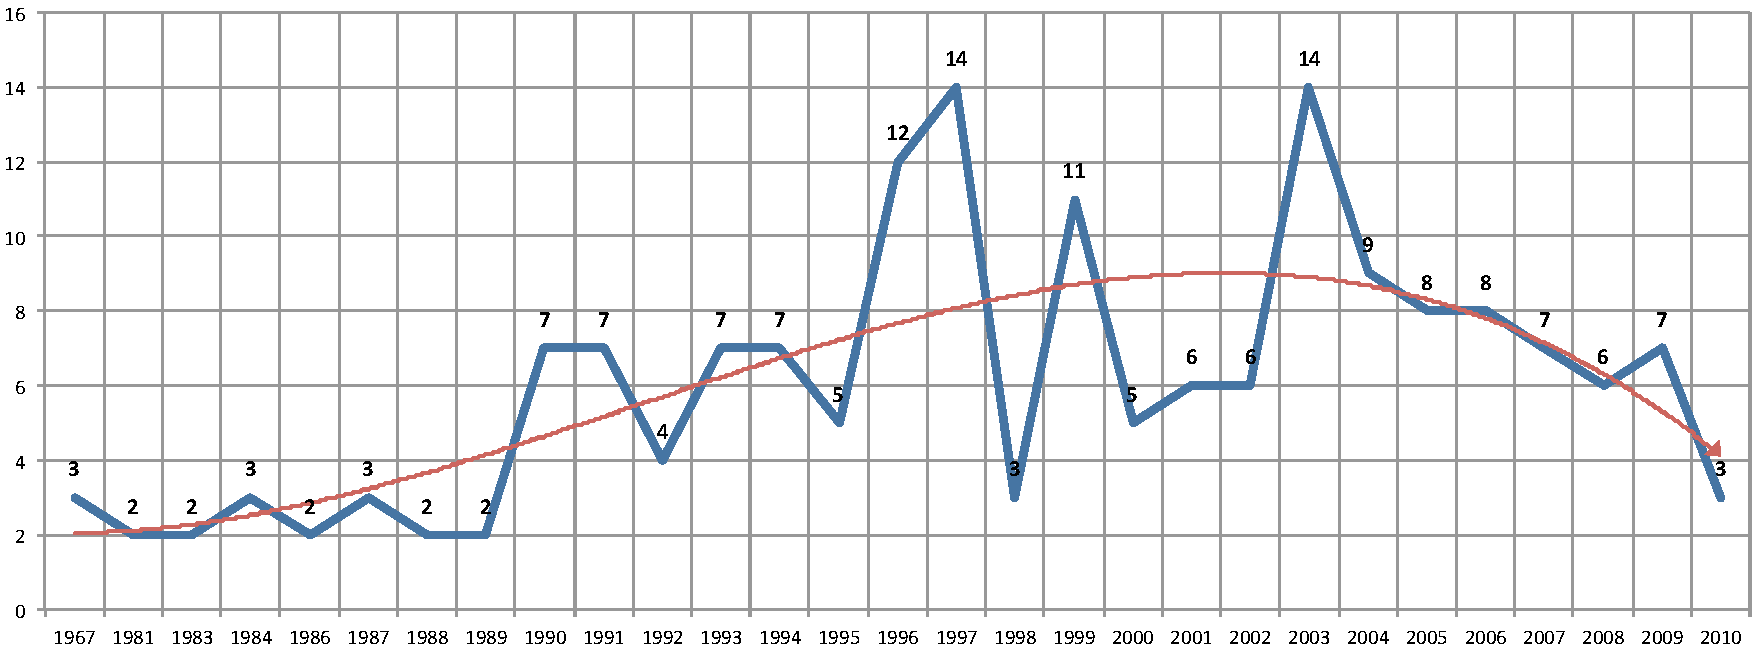
\includegraphics[scale=0.5]{abntex2-modelo-img-grafico.pdf}
	\end{center}
	\legend{Fonte: \citeonline[p. 24]{araujo2012}}
\end{figure}

% ---
\subsection{Figuras em \emph{minipages}}
% ---

\emph{Minipages} são usadas para inserir textos ou outros elementos em quadros
com tamanhos e posições controladas. Veja o exemplo da
\autoref{fig_minipage_imagem1} e da \autoref{fig_minipage_grafico2}.

\begin{figure}[htb]
 \label{teste}
 \centering
  \begin{minipage}{0.45\textwidth}
    \centering
    \caption{Imagem 1 da minipage} \label{fig_minipage_imagem1}
    
\includegraphics[scale=0.9]{abntex2-modelo-img-marca.pdf}
    \legend{Fonte: Produzido pelos autores}
  \end{minipage}
  \hfill
  \begin{minipage}{0.45\textwidth}
    \centering
    \caption{Grafico 2 da minipage} \label{fig_minipage_grafico2}
    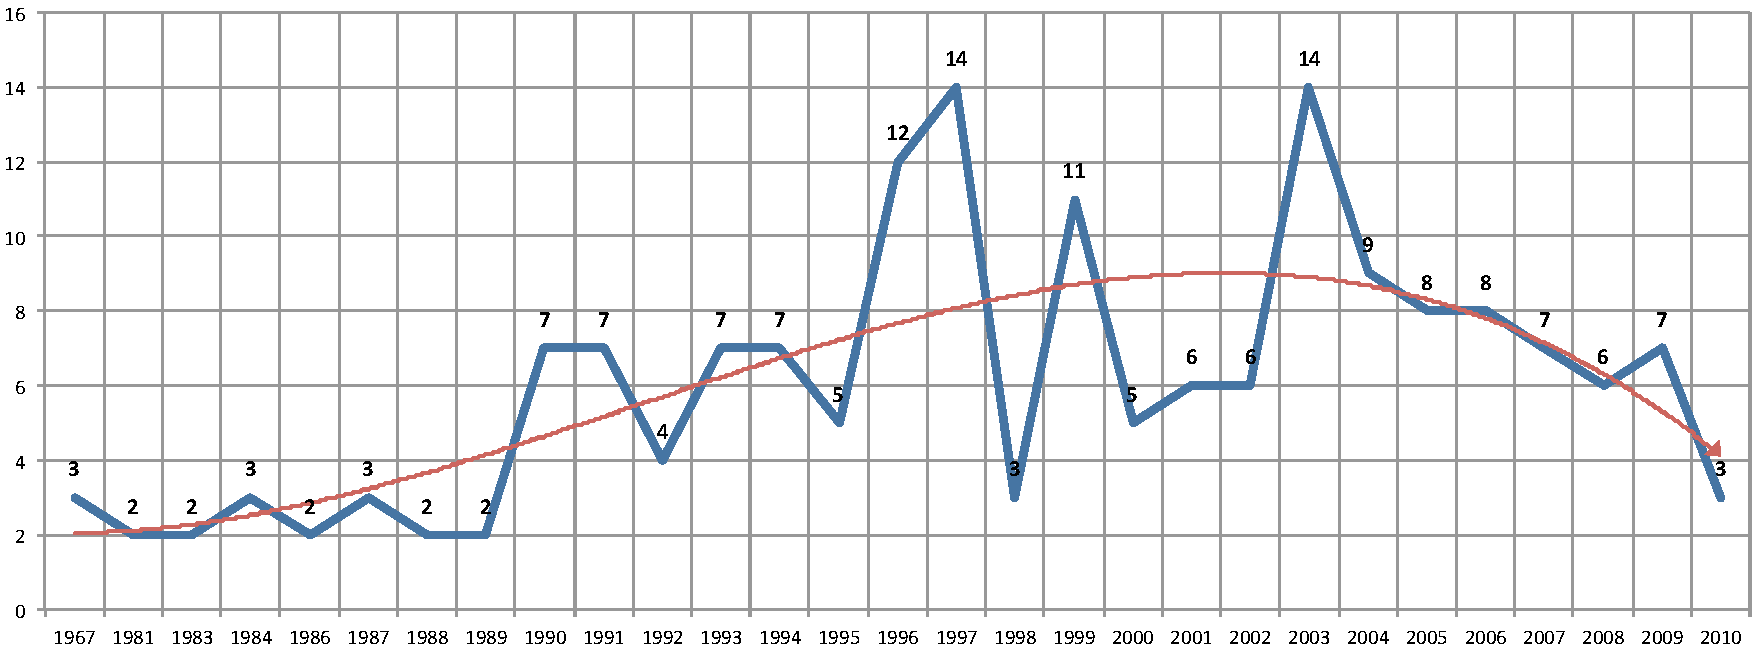
\includegraphics[scale=0.2]{abntex2-modelo-img-grafico.pdf}
    \legend{Fonte: \citeonline[p. 24]{araujo2012}}
  \end{minipage}
\end{figure}

Observe que, segundo a \citeonline[seções 4.2.1.10 e 5.8]{NBR14724:2011}, as
ilustrações devem sempre ter numeração contínua e única em todo o documento:

\begin{citacao}
Qualquer que seja o tipo de ilustração, sua identificação aparece na parte
superior, precedida da palavra designativa (desenho, esquema, fluxograma,
fotografia, gráfico, mapa, organograma, planta, quadro, retrato, figura,
imagem, entre outros), seguida de seu número de ordem de ocorrência no texto,
em algarismos arábicos, travessão e do respectivo título. Após a ilustração, na
parte inferior, indicar a fonte consultada (elemento obrigatório, mesmo que
seja produção do próprio autor), legenda, notas e outras informações
necessárias à sua compreensão (se houver). A ilustração deve ser citada no
texto e inserida o mais próximo possível do trecho a que se
refere. \cite[seções 5.8]{NBR14724:2011}
\end{citacao}

% ---
\section{Expressões matemáticas}
% ---

\index{expressões matemáticas}Use o ambiente \texttt{equation} para escrever
expressões matemáticas numeradas:

\begin{equation}
  \forall x \in X, \quad \exists \: y \leq \epsilon
\end{equation}

Escreva expressões matemáticas entre \$ e \$, como em $ \lim_{x \to \infty}
\exp(-x) = 0 $, para que fiquem na mesma linha.

Também é possível usar colchetes para indicar o início de uma expressão
matemática que não é numerada.

\[
\left|\sum_{i=1}^n a_ib_i\right|
\le
\left(\sum_{i=1}^n a_i^2\right)^{1/2}
\left(\sum_{i=1}^n b_i^2\right)^{1/2}
\]

Consulte mais informações sobre expressões matemáticas em
\url{https://code.google.com/p/abntex2/wiki/Referencias}.

% ---
\section{Enumerações: alíneas e subalíneas}
% ---

\index{alíneas}\index{subalíneas}\index{incisos}Quando for necessário enumerar
os diversos assuntos de uma seção que não possua título, esta deve ser
subdividida em alíneas \cite[4.2]{NBR6024:2012}:

\begin{alineas}

  \item os diversos assuntos que não possuam título próprio, dentro de uma mesma
  seção, devem ser subdivididos em alíneas; 
  
  \item o texto que antecede as alíneas termina em dois pontos;
  \item as alíneas devem ser indicadas alfabeticamente, em letra minúscula,
  seguida de parêntese. Utilizam-se letras dobradas, quando esgotadas as
  letras do alfabeto;

  \item as letras indicativas das alíneas devem apresentar recuo em relação à
  margem esquerda;

  \item o texto da alínea deve começar por letra minúscula e terminar em
  ponto-e-vírgula, exceto a última alínea que termina em ponto final;

  \item o texto da alínea deve terminar em dois pontos, se houver subalínea;

  \item a segunda e as seguintes linhas do texto da alínea começa sob a
  primeira letra do texto da própria alínea;
  
  \item subalíneas \cite[4.3]{NBR6024:2012} devem ser conforme as alíneas a
  seguir:

  \begin{alineas}
     \item as subalíneas devem começar por travessão seguido de espaço;

     \item as subalíneas devem apresentar recuo em relação à alínea;

     \item o texto da subalínea deve começar por letra minúscula e terminar em
     ponto-e-vírgula. A última subalínea deve terminar em ponto final, se não
     houver alínea subsequente;

     \item a segunda e as seguintes linhas do texto da subalínea começam sob a
     primeira letra do texto da própria subalínea.
  \end{alineas}
  
  \item no \abnTeX\ estão disponíveis os ambientes \texttt{incisos} e
  \texttt{subalineas}, que em suma são o mesmo que se criar outro nível de
  \texttt{alineas}, como nos exemplos à seguir:
  
  \begin{incisos}
    \item \textit{Um novo inciso em itálico};
  \end{incisos}
  
  \item Alínea em \textbf{negrito}:
  
  \begin{subalineas}
    \item \textit{Uma subalínea em itálico};
    \item \underline{\textit{Uma subalínea em itálico e sublinhado}}; 
  \end{subalineas}
  
  \item Última alínea com \emph{ênfase}.
  
\end{alineas}

% ---
\section{Espaçamento entre parágrafos e linhas}
% ---

\index{espaçamento!dos parágrafos}O tamanho do parágrafo, espaço entre a margem
e o início da frase do parágrafo, é definido por:

\begin{verbatim}
   \setlength{\parindent}{1.3cm}
\end{verbatim}

\index{espaçamento!do primeiro parágrafo}Por padrão, não há espaçamento no
primeiro parágrafo de cada início de divisão do documento
(\autoref{sec-divisoes}). Porém, você pode definir que o primeiro parágrafo
também seja indentado, como é o caso deste documento. Para isso, apenas inclua o
pacote \textsf{indentfirst} no preâmbulo do documento:

\begin{verbatim}
   \usepackage{indentfirst}      % Indenta o primeiro parágrafo de cada seção.
\end{verbatim}

\index{espaçamento!entre os parágrafos}O espaçamento entre um parágrafo e outro
pode ser controlado por meio do comando:

\begin{verbatim}
  \setlength{\parskip}{0.2cm}  % tente também \onelineskip
\end{verbatim}

\index{espaçamento!entre as linhas}O controle do espaçamento entre linhas é
definido por:

\begin{verbatim}
  \OnehalfSpacing       % espaçamento um e meio (padrão); 
  \DoubleSpacing        % espaçamento duplo
  \SingleSpacing        % espaçamento simples	
\end{verbatim}

Para isso, também estão disponíveis os ambientes:

\begin{verbatim}
  \begin{SingleSpace} ...\end{SingleSpace}
  \begin{Spacing}{hfactori} ... \end{Spacing}
  \begin{OnehalfSpace} ... \end{OnehalfSpace}
  \begin{OnehalfSpace*} ... \end{OnehalfSpace*}
  \begin{DoubleSpace} ... \end{DoubleSpace}
  \begin{DoubleSpace*} ... \end{DoubleSpace*} 
\end{verbatim}

Para mais informações, consulte \citeonline[p. 47-52 e 135]{memoir}.

% ---
\section{Inclusão de outros arquivos}\label{sec-include}
% ---

É uma boa prática dividir o seu documento em diversos arquivos, e não
apenas escrever tudo em um único. Esse recurso foi utilizado neste
documento. Para incluir diferentes arquivos em um arquivo principal,
de modo que cada arquivo incluído fique em uma página diferente, utilize o
comando:

\begin{verbatim}
   \include{documento-a-ser-incluido}      % sem a extensão .tex
\end{verbatim}

Para incluir documentos sem quebra de páginas, utilize:

\begin{verbatim}
   \input{documento-a-ser-incluido}      % sem a extensão .tex
\end{verbatim}

% ---
\section{Compilar o documento \LaTeX}
% ---

Geralmente os editores \LaTeX, como o
TeXlipse\footnote{\url{http://texlipse.sourceforge.net/}}, o
Texmaker\footnote{\url{http://www.xm1math.net/texmaker/}}, entre outros,
compilam os documentos automaticamente, de modo que você não precisa se
preocupar com isso.

No entanto, você pode compilar os documentos \LaTeX usando os seguintes
comandos, que devem ser digitados no \emph{Prompt de Comandos} do Windows ou no
\emph{Terminal} do Mac ou do Linux:

\begin{verbatim}
   pdflatex ARQUIVO_PRINCIPAL.tex
   bibtex ARQUIVO_PRINCIPAL.aux
   makeindex ARQUIVO_PRINCIPAL.idx 
   makeindex ARQUIVO_PRINCIPAL.nlo -s nomencl.ist -o ARQUIVO_PRINCIPAL.nls
   pdflatex ARQUIVO_PRINCIPAL.tex
   pdflatex ARQUIVO_PRINCIPAL.tex
\end{verbatim}

% ---
\section{Remissões internas}
% ---

Ao nomear a \autoref{tab-nivinv} e a \autoref{fig_circulo}, apresentamos um
exemplo de remissão interna, que também pode ser feita quando indicamos o
\autoref{cap_exemplos}, que tem o nome \emph{\nameref{cap_exemplos}}. O número
do capítulo indicado é \ref{cap_exemplos}, que se inicia à
\autopageref{cap_exemplos}\footnote{O número da página de uma remissão pode ser
obtida também assim:
\pageref{cap_exemplos}.}.
Veja a \autoref{sec-divisoes} para outros exemplos de remissões internas entre
seções, subseções e subsubseções.

O código usado para produzir o texto desta seção é:

\begin{verbatim}
Ao nomear a \autoref{tab-nivinv} e a \autoref{fig_circulo}, apresentamos um
exemplo de remissão interna, que também pode ser feita quando indicamos o
\autoref{cap_exemplos}, que tem o nome \emph{\nameref{cap_exemplos}}. O número
do capítulo indicado é \ref{cap_exemplos}, que se inicia à
\autopageref{cap_exemplos}\footnote{O número da página de uma remissão pode ser
obtida também assim:
\pageref{cap_exemplos}.}.
Veja a \autoref{sec-divisoes} para outros exemplos de remissões internas entre
seções, subseções e subsubseções.
\end{verbatim}

% ---
\section{Divisões do documento: seção}\label{sec-divisoes}
% ---

Esta seção testa o uso de divisões de documentos. Esta é a
\autoref{sec-divisoes}. Veja a \autoref{sec-divisoes-subsection}.

\subsection{Divisões do documento: subseção}\label{sec-divisoes-subsection}

Isto é uma subseção. Veja a \autoref{sec-divisoes-subsubsection}, que é uma
\texttt{subsubsection} do \LaTeX, mas é impressa chamada de ``subseção'' porque
no Português não temos a palavra ``subsubseção''.

\subsubsection{Divisões do documento: subsubseção}
\label{sec-divisoes-subsubsection}

Isto é uma subsubseção.

\subsubsection{Divisões do documento: subsubseção}

Isto é outra subsubseção.

\subsection{Divisões do documento: subseção}\label{sec-exemplo-subsec}

Isto é uma subseção.

\subsubsection{Divisões do documento: subsubseção}

Isto é mais uma subsubseção da \autoref{sec-exemplo-subsec}.


\subsubsubsection{Esta é uma subseção de quinto nível}\label{sec-exemplo-subsubsubsection}

Esta é uma seção de quinto nível. Ela é produzida com o seguinte comando:

\begin{verbatim}
\subsubsubsection{Esta é uma subseção de quinto
nível}\label{sec-exemplo-subsubsubsection}
\end{verbatim}

\subsubsubsection{Esta é outra subseção de quinto nível}\label{sec-exemplo-subsubsubsection-outro}

Esta é outra seção de quinto nível.


\paragraph{Este é um parágrafo numerado}\label{sec-exemplo-paragrafo}

Este é um exemplo de parágrafo nomeado. Ele é produzida com o comando de
parágrafo:

\begin{verbatim}
\paragraph{Este é um parágrafo nomeado}\label{sec-exemplo-paragrafo}
\end{verbatim}

A numeração entre parágrafos numeradaos e subsubsubseções são contínuas.

\paragraph{Esta é outro parágrafo numerado}\label{sec-exemplo-paragrafo-outro}

Esta é outro parágrafo nomeado.

% ---
\section{Este é um exemplo de nome de seção longo. Ele deve estar
alinhado à esquerda e a segunda e demais linhas devem iniciar logo abaixo da
primeira palavra da primeira linha}
% ---

Isso atende à norma \citeonline[seções de 5.2.2 a 5.2.4]{NBR14724:2011} 
 e \citeonline[seções de 3.1 a 3.8]{NBR6024:2012}.

% ---
\section{Diferentes idiomas e hifenizações}
\label{sec-hifenizacao}
% ---

Para usar hifenizações de diferentes idiomas, inclua nas opções do documento o
nome dos idiomas que o seu texto contém. Por exemplo (para melhor
visualização, as opções foram quebras em diferentes linhas):

\begin{verbatim}
\documentclass[
	12pt,
	openright,
	twoside,
	a4paper,
	english,
	french,
	spanish,
	brazil
	]{abntex2}
\end{verbatim}

O idioma português-brasileiro (\texttt{brazil}) é incluído automaticamente pela
classe \textsf{abntex2}. Porém, mesmo assim a opção \texttt{brazil} deve ser
informada como a última opção da classe para que todos os pacotes reconheçam o
idioma. Vale ressaltar que a última opção de idioma é a utilizada por padrão no
documento. Desse modo, caso deseje escrever um texto em inglês que tenha
citações em português e em francês, você deveria usar o preâmbulo como abaixo:

\begin{verbatim}
\documentclass[
	12pt,
	openright,
	twoside,
	a4paper,
	french,
	brazil,
	english
	]{abntex2}
\end{verbatim}

A lista completa de idiomas suportados, bem como outras opções de hifenização,
estão disponíveis em \citeonline[p.~5-6]{babel}.

Exemplo de hifenização em inglês\footnote{Extraído de:
\url{http://en.wikibooks.org/wiki/LaTeX/Internationalization}}:

\begin{otherlanguage*}{english}
\textit{Text in English language. This environment switches all language-related
definitions, like the language specific names for figures, tables etc. to the other
language. The starred version of this environment typesets the main text
according to the rules of the other language, but keeps the language specific
string for ancillary things like figures, in the main language of the document.
The environment hyphenrules switches only the hyphenation patterns used; it can
also be used to disallow hyphenation by using the language name
`nohyphenation'.}
\end{otherlanguage*}

Exemplo de hifenização em francês\footnote{Extraído de:
\url{http://bigbrowser.blog.lemonde.fr/2013/02/17/tu-ne-tweeteras-point-le-vatican-interdit-aux-cardinaux-de-tweeter-pendant-le-conclave/}}:

\begin{otherlanguage*}{french}
\textit{Texte en français. Pas question que Twitter ne vienne faire une
concurrence déloyale à la traditionnelle fumée blanche qui marque l'élection
d'un nouveau pape. Pour éviter toute fuite précoce, le Vatican a donc pris un
peu d'avance, et a déjà interdit aux cardinaux qui prendront part au vote
d'utiliser le réseau social, selon Catholic News Service. Une mesure valable
surtout pour les neuf cardinaux – sur les 117 du conclave – pratiquants très
actifs de Twitter, qui auront interdiction pendant toute la période de se
connecter à leur compte.}
\end{otherlanguage*}

Pequeno texto em espanhol\footnote{Extraído de:
\url{http://internacional.elpais.com/internacional/2013/02/17/actualidad/1361102009_913423.html}}:

\foreignlanguage{spanish}{\textit{Decenas de miles de personas ovacionan al pontífice en su
penúltimo ángelus dominical, el primero desde que anunciase su renuncia. El Papa se
centra en la crítica al materialismo}}.

O idioma geral do texto por ser alterado como no exemplo seguinte:

\begin{verbatim}
  \selectlanguage{english}
\end{verbatim}

Isso altera automaticamente a hifenização e todos os nomes constantes de
referências do documento para o idioma inglês. Consulte o manual da classe
\cite{abntex2classe} para obter orientações adicionais sobre internacionalização de
documentos produzidos com \abnTeX.

A \autoref{sec-citacao} descreve o ambiente \texttt{citacao} que pode receber
como parâmetro um idioma a ser usado na citação.

% ---
\section{Consulte o manual da classe \textsf{abntex2}}
% ---

Consulte o manual da classe \textsf{abntex2} \cite{abntex2classe} para uma
referência completa das macros e ambientes disponíveis. 

Além disso, o manual possui informações adicionais sobre as normas ABNT
observadas pelo \abnTeX\ e considerações sobre eventuais requisitos específicos
não atendidos, como o caso da \citeonline[seção 5.2.2]{NBR14724:2011}, que
especifica o espaçamento entre os capítulos e o início do texto, regra
propositalmente não atendida pelo presente modelo.

% ---
\section{Referências bibliográficas}
% ---

A formatação das referências bibliográficas conforme as regras da ABNT são um
dos principais objetivos do \abnTeX. Consulte os manuais
\citeonline{abntex2cite} e \citeonline{abntex2cite-alf} para obter informações
sobre como utilizar as referências bibliográficas.

%-
\subsection{Acentuação de referências bibliográficas}
%-

Normalmente não há problemas em usar caracteres acentuados em arquivos
bibliográficos (\texttt{*.bib}). Porém, como as regras da ABNT fazem uso quase
abusivo da conversão para letras maiúsculas, é preciso observar o modo como se
escreve os nomes dos autores. Na ~\autoref{tabela-acentos} você encontra alguns
exemplos das conversões mais importantes. Preste atenção especial para `ç' e `í'
que devem estar envoltos em chaves. A regra geral é sempre usar a acentuação
neste modo quando houver conversão para letras maiúsculas.

\begin{table}[htbp]
\caption{Tabela de conversão de acentuação.}
\label{tabela-acentos}

\begin{center}
\begin{tabular}{ll}\hline\hline
acento & \textsf{bibtex}\\
à á ã & \verb+\`a+ \verb+\'a+ \verb+\~a+\\
í & \verb+{\'\i}+\\
ç & \verb+{\c c}+\\
\hline\hline
\end{tabular}
\end{center}
\end{table}


% ---
\section{Precisa de ajuda?}
% ---

Consulte a FAQ com perguntas frequentes e comuns no portal do \abnTeX:
\url{https://code.google.com/p/abntex2/wiki/FAQ}.

Inscreva-se no grupo de usuários \LaTeX:
\url{http://groups.google.com/group/latex-br}, tire suas dúvidas e ajude
outros usuários.

Participe também do grupo de desenvolvedores do \abnTeX:
\url{http://groups.google.com/group/abntex2} e faça sua contribuição à
ferramenta.

% ---
\section{Você pode ajudar?}
% ---

Sua contribuição é muito importante! Você pode ajudar na divulgação, no
desenvolvimento e de várias outras formas. Veja como contribuir com o \abnTeX\
em \url{https://code.google.com/p/abntex2/wiki/ComoContribuir}.

% ---
\section{Quer customizar os modelos do \abnTeX\ para sua instituição ou
universidade?}
% ---

Veja como customizar o \abnTeX\ em:
\url{https://code.google.com/p/abntex2/wiki/ComoCustomizar}.



\chapter{Conclusão e Trabalhos Futuros }\label{chap:conclusão}

\section{Conclusão}

As discussões sobre sustentabilidade estão ampliando seu alcance e chegando em áreas diversas, levando a novas práticas e ampla conscientização, mas nem sempre com a rapidez esperada.

A indústria de equipamentos e dispositivos eletroeletrônicos tem produzido novidades de forma constante, gerando inovação tecnológica em equipamentos e práticas  cotidianas, e ao final do tempo de vida útil destes equipamentos uma quantidade de resíduos considerável.

Neste sentido, espera-se que os utilizadores, em pequena ou larga escala, sejam responsáveis ao utilizar estes recursos, a fim de utilizar corretamente e pelo maior tempo possível todos os recursos tecnológicos disponíveis para sua utilização pessoal ou profissional.

O estudo de caso realizado na UESB, apontou mesmo realizando algumas práticas verdes, como virtualização e Gestão Eletrônica de Documentos, existe uma grande necessidade de se investir em TI Verde, como a criação de estrategias e planos ambientais, implementação de um SGA, criação de uma semana anual para divulgar e discutir a sustentabilidade em todos os âmbitos, entre outras.

Se mostrou importante a criação das propostas apresentadas no presente trabalho, e caso as mesmas forem implementadas, teremos um grande avanço em relação ao que foi analisado, podendo incentivar outras organizações, sendo elas públicas ou privadas, a se tornarem sustentáveis, investindo em gestão ambiental e a preservação do meio ambiente, garantindo um futuro melhor para as gerações futuras.

Para finalizar, a partir do desenvolvimento deste trabalho, notou-se que existe a possibilidade de se ampliar o estudo para outras pesquisas. Estas possibilidades são apresentadas como trabalhos futuros.


%A realização do presente trabalho foi de grande relevância para aumentar os conhecimentos do autor sobre a necessidade de aplicar as práticas de TI Verde. Discutir aspectos relacionado aos impactos ambientais, causados pela má utilização da tecnologia, é de suma importância para a preservação do meio ambiente, garantindo um futuro melhor para as gerações futuras.

%Devido a grande influência que a UESB possui na comunidade local, existe uma preocupação em relação a aplicação da TI Verde, sendo importante identificar se a mesma otimiza o uso das tecnologias, de maneira que contribua com a sustentabilidade e o desenvolvimento sustentável. Com isso é necessário realizar um estudo sobre  TI Verde, para poder analisar a UINFOR, setor responsável pela TI, com intuito de propor melhorias e novas soluções.

%Partindo do objetivo de conscientizar a UESB sobre a importância das práticas sustentáveis na utilização da tecnologia, foi feito um longo estudo para ter um grande embasamento teórico, que serviu para poder avaliar o uso da TI Verde, identificando que a UESB implementa práticas como a Virtualização e o projeto de GED. Foram propostos soluções como a criação de estrategias e planos ambientais, implementação de um SGA, criação de uma semana anual para divulgar e discutir a sustentabilidade em todos os âmbitos, entre outras.


%Com relação às dificuldades para o desenvolvimento do trabalho, o referencial teórico foi a etapa mais difícil do estudo. Pois assunto estudado é bastante amplo, possuindo diversos tópicos. Além disso, foi consultado vários autores e trabalhos diferentes, para um melhor entendimento e compreensão do tema.

%Quanto ao levantamento de dados foi uma etapa tranquila, pelo fato de já possuir uma proximidade e conhecimento dos processos e da estado em que a UESB se encontrava em relação a utilização da TI Verde.

%A situação atual quanto à utilização  da TI Verde pela UESB foi melhor do que a esperado, mesmo assim existe vários pontos que ela precisa se adequar para poder ser considerada uma instituição sustentável.

%As propostas sugeridas foram de fácil implementação e, mesmo com o baixo orçamento da instituição, elas podem ser utilizadas, tendo uma redução nos gastos a curto prazo. O dinheiro economizado poderia então ser investido em em outros projetos.

%Finalizando, o presente trabalho se demonstra de grande importância e de grande contribuição para que a UESB se torne uma organização sustentável, cumprindo com a sua responsabilidade social, além de abrir caminho para que as demais organizações, sendo elas públicas ou privadas de qualquer setor, também possam implementar práticas verdes.

\section{Trabalhos futuros}

Como possíveis trabalhos futuros, pode-se apontar:

\begin{itemize}
\item Ampliar o estudo para toda a UESB, analisando também os campi de Jequié e Itapetinga, englobando outros pontos da sustentabilidade, além da TI Verde;
\item Propor um modelo de Tecnologia da Informação Verde e  um Sistema de Gestão Ambienta para serem implementados na UESB;
\item Realizar o mesmo estudo nas demais instituições de ensino superior de Vitória da Conquista, como o Instituto Federal da Bahia (IFBA), Universidade Federal da Bahia (UFBA), Faculdade de Tecnologia e Ciências (FTC) e Faculdade Independente do Nordeste (FAINOR).
\end{itemize}




% ----------------------------------------------------------
% Finaliza a parte no bookmark do PDF para que se inicie o bookmark na raiz e adiciona espaço de parte no Sumário
% ----------------------------------------------------------
\phantompart


% ----------------------------------------------------------
% ELEMENTOS PÓS-TEXTUAIS
% ----------------------------------------------------------
\postextual

% Referências bibliográficas
\bibliography{bibtex/referencias}
%\addbibresource{bibtex/referencias.bib}  

% Apêndices
% Apêndices
% ---
% Inicia os apêndices
% ---
\begin{apendicesenv}

% Imprime uma página indicando o início dos apêndices
\partapendices

% ----------------------------------------------------------
\chapter{Quisque libero justo}
% ----------------------------------------------------------

\lipsum[50]

% ----------------------------------------------------------
\chapter{Nullam elementum urna vel imperdiet sodales elit ipsum pharetra ligula
ac pretium ante justo a nulla curabitur tristique arcu eu metus}
% ----------------------------------------------------------
\lipsum[55-57]

\end{apendicesenv}
% ---


% Anexos
%% ----------------------------------------------------------
% Anexos
% ---
% Inicia os anexos
% ---
\begin{anexosenv}

% Imprime uma página indicando o início dos anexos
\partanexos

% ---
\chapter{Morbi ultrices rutrum lorem.}
% ---
\lipsum[30]

% ---
\chapter{Cras non urna sed feugiat cum sociis natoque penatibus et magnis dis
parturient montes nascetur ridiculus mus}
% ---

\lipsum[31]

% ---
\chapter{Fusce facilisis lacinia dui}
% ---

\lipsum[32]

\end{anexosenv}


%---------------------------------------------------------------------
% INDICE REMISSIVO
%---------------------------------------------------------------------
\phantompart
\printindex
%---------------------------------------------------------------------

\end{document}
